\documentclass[12pt,a4paper]{scrartcl}


\usepackage{graphicx}
\usepackage{amsmath}
\usepackage{amsfonts}
\usepackage{amssymb}
\linespread{1.15}
\usepackage[margin=2.3cm]{geometry}
\usepackage{xcolor}
\usepackage{adjustbox}
\usepackage{subcaption}
\numberwithin{equation}{section}
\numberwithin{table}{section}
\numberwithin{figure}{section}

\usepackage{bm}
\let\mathbf\bm
\newcommand{\m}[1]{\mathrm{#1}}
\newcommand{\tn}[1]{\textnormal{#1}}
\newcommand{\pd}[2]{\frac{\partial{#1}}{\partial{#2}}}
\newcommand{\rec}[1]{\frac{1}{#1}}
\newcommand{\md}[2]{\frac{\mathrm{d}{#1}}{\mathrm{d}{#2}}}
\newcommand{\z}[1]{\left({#1}\right)}
\newcommand{\sz}[1]{\left[{#1}\right]}
\newcommand{\kz}[1]{\left\{{#1}\right\}}
\newcommand{\follows}{\quad\Rightarrow\quad}
\newcommand{\equivalent}{\quad\Leftrightarrow\quad}
\newcommand{\mom}{\mathbf p}
\newcommand{\prob}{\mathtt p}
\newcommand{\pres}{\mathsf p}
\newcommand\newsubcap[1]{\phantomcaption%
       \caption*{\thefigure\thesubfigure~\figurename: #1}}


\usepackage[T1]{fontenc}
\usepackage[utf8]{inputenc}
\usepackage[magyar]{babel}
\usepackage{lmodern}

\usepackage{placeins}	%FloatBarrier parancs, a figure előtti szöveget nem ír ki, amíg a képet sikeresen be nem ágyazza
\usepackage{subcaption}	%alábra lehetősége
\usepackage{epstopdf}
\usepackage{xcolor}
\usepackage[hidelinks,unicode]{hyperref}
\hypersetup{
    colorlinks,
    linkcolor={red!50!black},
    citecolor={blue!50!black},
    urlcolor={blue!80!black}
}

\usepackage{cleveref}	




\begin{document}
\title{Hőtan és folytonos közegek mechanikája\\(emelt szint)}
\author{hotanef19va, Anyagfizikai Tanszék\\
Előadás: Ispánovity Péter Dusán\\
Gyakorlat: Tüzes Dániel}
\maketitle
\tableofcontents
\section*{Mi ez?}
A 2019/2020-as tanévtől kezdődően a hőtan és folytonos közegek mechanikája egy tárgyban kerül meghirdetésre. A téma a szemeszter első felében elsősorban a folytonos közegek mechanikája, második felében a hőtan. Ez a jegyzet az előadáshoz és a gyakorlathoz közösen írt tananyag, amely a hőtan részt fedezi. További támogató anyagok esetleg elérhetőek az ELTE Canvas rendszerében (mint pl.\ előadás videók), az
\href{http://ispanovity.web.elte.hu/teaching/}{előadó} vagy a  \href{http://metal.elte.hu/~tuzes/oktatas/#folytkoz_19_20}{gyakorlatvezető} honlapján (mint pl.\ házi feladatok).

Külön köszönet illeti meg Boldizsár Bálint hallgatót, aki nemcsak az előadáshoz tartozó demonstrációban, de ennek a jegyzetnek az elkészítésében is szerepet vállalt.

\pagebreak

\section{A termodinamika alapfogalmai}

\emph{A termodinamika tárgya; Hőmérsékletmérés: skálák, feltevések; Ideális gáz: Boyle--Mariotte és Gay--Lussac kísérletei és törvényei, állapotegyenlet; Kelvin-skála; Termodinamikai rendszer fogalma;
Egyszerű rendszerek; Állapotjelzők és osztályozásuk; Termodinamikai egyensúly és 0.~főtétel}

Számtalan olyan jelenség van, ahol a hőmérsékletnek szerepe van; a termodinamika ilyen folyamatokat illetve rendszereket vizsgál. \emph{Termodinamikai rendszer}ről beszélünk, amikor
\begin{itemize}
    \item a rendszer mérete sokkal nagyobb, mint az alkotó részecskéké,
    \item a benne lezajló bonyolult folyamatokat nem akarjuk részletesen leírni\footnote{\,Tipikusan $10^{23}$ db.~részecskét kellene leírni, azonban ez sem analitikusan, sem numerikusan nem kezelhető. Nagy részecskeszámú rendszereket molekuladinamikai szimulációkkal szokás vizsgálni, jelenleg pár milliárd ($\sim10^9$) részecske modellezése lehetséges.}, mert a makroszkópikusan is vizsgálható mennyiségek enélkül is megérthetőek.
\end{itemize}
A termodinamikát úgy vezettük be, hogy a \emph{hőmérséklettel} kapcsolatos jelenségeket tárgyalja, azonban nem olyan egyszerű fenomenologikusan megfogalmazni\footnote{\,Statisztikus fizikai módon egy fokkal korrektebbül lesz definiálható, erre még a későbbiekben röviden visszatérünk.}, hogy mi is pontosan a hőmérséklet. Itt a kiindulópontunk saját elemi érzékszervi tapasztalataink, melyek segítségével meg tudjuk különböztetni a hideget a melegtől. A hőmérséklettől, mint fizikai mennyiségtől azt várjuk el, hogy a test hőállapotát jellemzze olyan módon, hogy a hidegebb illetve melegebb testekhez mérőszámot rendeljen, és ezeket a hidegtől a meleg felé nőve úgy rendezze sorba, hogy az megegyezzen érzékszervi tapasztalatainkkal. Ilyen módon \emph{hőmérsékleti skálákat} definiálhatunk. Fontos tapasztalat a hőmérséklet bevezetéséhez, hogy
\begin{itemize}
    \item adott stacionárius környezetben a test hőfoka állandósul, amit a környezete szab meg,
    \item az érintkezésbe hozott testek (termikus kölcsönhatás) hőfoka kiegyenlítődik.
\end{itemize}
A hőmérsékletmérést olyan fizikai folyamatok teszik lehetővé, melyek során a hőmérsékletváltozás egy másik fizikai mennyiség (pl.~hosszúság) megváltozását eredményezi. Ilyen folyamatok pl.:
\begin{itemize}
    \item \emph{Fázisátalakulás:} így definiálta 1742-ben Celsius\footnote{\,Anders Celsius, 1701-1744.} a róla elnevezett hőmérsékletskálát, ahol a víz olvadás- és forráspontja segítségével 100-as beosztású hőmérsékleti skálát készített.
    \item \emph{Hőtágulás:} ilyen módon működnek a folyadékhőmérők (pl.~higany, alkohol), ugyanis különböző hőmérsékleten a testek térfogata eltérő, az alkalmazott folyadékok esetében pedig a hőtágulás mértéke a vizsgált tartományban közelítőleg lineáris. Szokás még alkalmazni ún.~bimetálokat is: ekkor két különböző anyagú fémet rögzítenek össze, melyek térfogata a hőmérséklet függvényében eltérő módon változik, így a bimetál elgörbül, melynek mértéke a hőtágulási együtthatók ismeretében megadható. Ez látható \aref{fig:termo_1_6}. ábrán.
    \begin{figure}
        \centering
        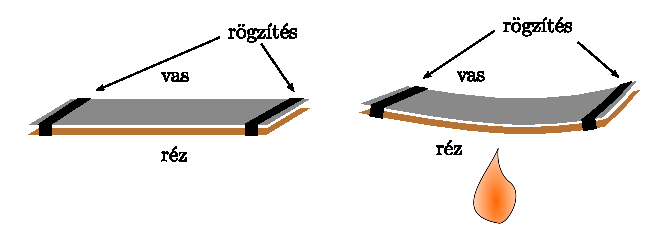
\includegraphics{termo_1/termo_1_6.eps}
        \caption{Bimetál, mely hő hatására elhajlik.}
        \label{fig:termo_1_6}
    \end{figure}.
    \item \emph{Termoelektromos jelenségek:} egyrészt ehhez kapcsolódik, hogy a vezetők ellenállásának is van hőmérsékletfüggése, mely például adott feszültség esetén az áram mérésével meghatározható. Alkalmaznak még termoelemeket is hőmérsékletmérésre. Ebben az esetben két különböző fémet helyeznek egymással kontaktusba, majd különböző hőmérsékletre felfűtik őket (Seebeck\footnote{\,Thomas Johann Seebeck, 1770-1831.}-effektus\footnote{\,Ez a transzportfolyamatok egyik kereszteffektusaként ismert, későbbi tanulmányaitok során az Onsager-relációk kapcsán is találkozni fogtok még vele.}).
    \item \emph{Infrasugárzás:} a test által kibocsátott infrasugárzás mértéke arányos a hőmérsékletével (Planck\footnote{\,Max Planck, 1858-1947.}-féle sugárzási törvény\footnote{\,A Planck-féle sugárzási törvény értelmében az időegység alatt kisugárzott energia: $E\propto T^4$.}). Hőkamera esetében a kamera ezt detektálja, majd színes képpé alakítja. Előnye, hogy a műszer és a mérendő test között nem szükséges a fizikai kontaktus, ezért a műszer egyáltalán nem változtatja meg a mérendő test tulajdonságait.
\end{itemize}
A hőmérsékletméréshez kell egyrészt a mérendő fizikai rendszer, a mérés kalibrációja, illetve referenciapont is. A hőmérsékletmérés feltevései a következők:
\begin{itemize}
    \item a termikus kölcsönhatás miatt a mérendő test és a mérőeszköz hőmérséklete kiegyenlítődik,
    \item a mérőeszköz csak elhanyagolható mértékben változtatja meg a rendszer hőmérsékletét.
\end{itemize}
Fontos megjegyezni még emelett, hogy minden módszer csak bizonyos tartományok között működik (pl.~az alkoholos hőmérők is adott hőmérséklet alatt megfagynak).

Említettük már, hogy hőmérsékleti skálákat lehet definiálni, melyek közül a leggyakoriabbak:
\begin{itemize}
    \item \emph{Celsius-skála:} 1742-ben alkotta meg Celsius. Eredetileg ő 0$^\circ$C-nak a víz forráspontját és 100$^\circ$C-nak a víz fagyáspontját határozta meg standard légköri nyomáson, a köztük lévő részt pedig egyenlő közönként 100 részre osztotta. Ma a skálát pont fordítva használjuk: a víz fagyáspontja 0$^\circ$C, míg a forráspontja 100$^\circ$C normál légköri nyomáson.
    \item \emph{Fahrenheit\footnote{\,Daniel Gabriel Fahrenheit, 1686-1736.}-skála:} 1724-ben alkotta meg Fahrenheit. Olyan hőmérsékleti skálát akart alkotni, ahol nincsenek negatív számok. 0$^\circ$F-nek a szülővárosában, Gda\'nskban, 1708 telén mért leghidegebb hőmérsékletet választotta (ami egy megfelelő telített sósvíz fagyáspontjával könnyen reprodukálható volt), 100$^\circ$F-nek pedig az emberi test normál, 37$^\circ$C-os hőmérsékletét választotta. Ekkor 32$^\circ$F a víz fagyáspontja míg 212$^\circ$F a víz forráspontja standard légköri nyomáson\footnote{\,A Celsius- illetve Fahrenheit-skálák közötti átváltás: $$T_C = \frac 59(T_F -32),\quad  T_F = \frac 95 T_C+32,$$ ahol $T_C$ és $T_F$ jelöli rendre a Celsius- illetve Fahrenheit-skálán mért hőmérsékleteket.}. Ma már csak az angolszász nyelvterületeken használatos.
    \item \emph{Kelvin\footnote{\,Lord Kelvin, Kelvin első bárója vagy William Thomson, 1824-1907.}-skála:} a fizikai számolások szempontjából ez a legfontosabb, a továbbiakban minden hőmérsékleti kifejezést ebben értünk, kivéve ha azt külön nem jelezzük. Ez az \emph{abszolút hőmérsékleti skála}. Az abszolút 0 fok: $0 \mathrm K = -273{,}16^\circ$C. Abszolút 0 fokon a részecskék nem végeznek hőmozgást, azonban a $0$K tetszőlegesen megközelíthető, de nem érhető el\footnote{\,Ezzel a termodinamika III.~főtétele kapcsán még részletesen is fogunk foglalkozni.}. Említettük már korábban, hogy a hőmérsékletméréshez referenciapont is szükséges, ami a Kelvin-skála esetében a $0$K és a víz ún.~hármaspontja\footnote{\,A víz hármaspontjának nevezzük, amikor a hőmérséklet $273{,}1575$K, a nyomás pedig $611{,}657$Pa, ekkor mindhárom halmazállapota (szilárd, folyadék, gáz) egyszerre vannak jelen.}; $1$K hőmérsékletkülönbség a víz hármaspontjának $1/273{,}16$-od része. Ennek megfelelően a két skála közötti átváltás: $T_K = T_C + 273{,}16$, ahol $T_K$ és $T_C$ jelöli rendre a Kelvin- illetve Celsius-skálán mért hőmérsékleteket.
\end{itemize}
A termodinamika tárgyalását könnyen kezelhető rendszerekkel kezdjük. \emph{Egyszerű termodinamikai rendszerről} beszélünk, ha
\begin{itemize}
    \item izotrop: nincs kitüntetett irány,
    \item homogén: nincs kitüntetett pont,
    \item nincsen semmilyen elektromágneses jelenség,
    \item a felületi jelenségek elhanyagolhatóak,
    \item két darab független állapotjelző van.
\end{itemize}
Állapotjelzőnek nevezzük az olyan fizikai mennyiségeket, melyek egy egyszerű termodinamikai rendszer esetén
\begin{itemize}
    \item jellemzik a rendszer makroszkópikus állapotát,
    \item egy állapotban egyértelműen meghatározottak,
    \item nem függenek a rendszer múltjától.
\end{itemize} 
Megjegyezzük, hogy végtelen sok állapotjelző van, ugyanis bármely két állapotjelző kombinációja is állapotjelző. Két csoportba lehet sorolni az állapotjelzőket: az \emph{extenzív állapotjelzők} additívak (összeadódnak), ilyen például a térfogat ($V$), a részecskeszám ($N$), a belső energia ($U$), az entrópia ($S$)\footnote{\,Ezekkel a későbbiekben még részletesen fogunk foglalkozni.}, míg az \emph{intenzív állapotjelzők} egyensúlyban kiegyenlítődnek, függetlenek a rendszer mennyiségétől; ilyen például a nyomás ($p$), a hőmérséklet ($T$) vagy a kémiai potenciál ($\mu$). Az állapotjelzők gyakran nem függetlenek egymástól, a köztük fennálló összefüggéseket \emph{állapotegyenleteknek} nevezzük. Ez utóbbiak tehát az állapotjelzők függvényei, melyek minden esetben az alábbi alakban írhatóak fel:
\begin{align}
    f(p,V,T,\dots)=0.
\end{align}
Az állapotegyenlet meghatározása alapvetően kísérleti úton történik és a vizsgált anyagra jellemző\footnote{Később meghatározható lesz a statisztikus fizika módszereivel is.}.

\emph{Termodinamikai egyensúlyról} beszélünk, ha a rendszer makroszkopikus tulajdonságai, és ezáltal az állapotjelzői időben állandóak. Legyen három rendszerünk, jelöljük őket A, B és C-vel. Fontos megállapítás, hogy ha A és B rendszer, illetve B és C rendszer is egyensúlyban vannak, akkor A és C rendszer is egyensúlyban vannak egymással, azaz ha termikus kapcsolatba kerülnek, akkor az nem okozza az állapotjelzők megváltozását. Ezt az axiómát hívjuk a \emph{termodinamika 0.~főtételének}.

Az egyik legfontosabb egyszerű termodinamikai rendszer az ún.~\emph{ideális gáz}. Ideális gázról beszélünk, ha:
\begin{itemize}
    \item a gázt alkotó atomok vagy molekulák térfogata a gáz által kitöltött térfogathoz képest elhanyagolható,
    \item a gázmolekulák egymással ütköznek, azonban más (taszító vagy vonzó) kölcsönhatásban egymással nem állnak,
    \item a gázmolekulák egymással illetve a fallal vett ütközése tökéletesen rugalmas,
    \item a gázmolekulák átlagos sebességét és kinetikus energiáját a gáz hőmérséklete szabja meg valamint
    \item az azonos hőmérsékleten, azonos számú gázmolekula kinetikus energiája megegyezik, és független a gáz anyagi minőségétől.
\end{itemize}
Három fontos kísérlet és ebből levont következtetés vonatkozik az ideális gázokra, melyekből az állapotegyenlete meghatározható.
\begin{itemize}
    \item \emph{Boyle\footnote{\,Robert Boyle, 1627-1691.}--Mariotte\footnote{\,Edme Mariotte 1620-1684.}-törvény:} 1669-ben fogalmazták meg, hogy állandó hőmérsékleten $pV = \textnormal{konst.}$, azaz a nyomás és a térfogat fordítottan arányosak egymással. Ennek igazolásához különböző nyomások mellett mérjük, hogy egy csőben lévő golyó mennyivel mozdul el, azaz hogyan változik meg a bezárt levező térfogata, ez látható \aref{fig:termo_1_4}. ábrán.
    \item \emph{Gay-Lussac\footnote{\,Joseph Louis Gay-Lussac, 1778-1850.} I.~törvénye:} 1802., állandó nyomáson melegítés hatására nő a gáz térfogata, mégpedig a hőmérséklet és a térfogat megváltozása között egyenes arányosság áll fent. Továbbá igaz, hogy:
    \begin{align}
        V(t) = V_0(1+\beta t),
    \end{align}
    ahol $V$ a térfogat, $V_0$ a $0^\circ$C-on mért térfogat, $\beta$ az ún.~térfogati hőtágulási együttható, $t$ pedig a $^\circ$C-ban mért hőmérséklet. \Aref{fig:termo_1_1}. ábrán látható, hogy a térfogat a hőmérsékletnek lineáris függvénye. 
    \begin{figure}[h!]
    \centering
    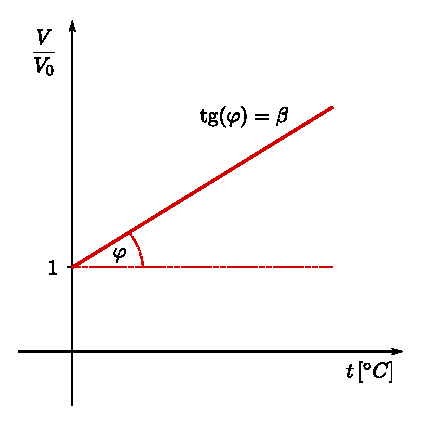
\includegraphics{termo_1/termo_1_1.eps}
    \caption{Gay-Lussac I. törvénye.}
    \label{fig:termo_1_1}
    \end{figure}
Ennek a méréséhez manométer segítségével mérjük különböző hőmérsékleteket a bezárt levegő térfogatának változását, mely során az U-alakú csőben lévő folyadékoszlop elmozdul. A kísérleti összeállítás látható \aref{fig:termo_1_5}. ábrán.
    \begin{figure}[!h]
    \centering
    \begin{subfigure}[t]{0.45\textwidth}
            \centering
            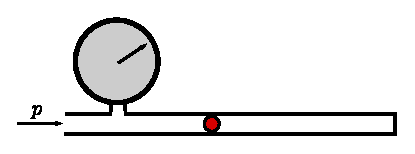
\includegraphics[width=\textwidth]{termo_1/termo_1_4}
            %\phantonsubcaption
            \newsubcap{Boyle--Mariotte-törvény kimérése}
            \label{fig:termo_1_4}
    \end{subfigure}\hfill
    \begin{subfigure}[t]{0.45\textwidth}
            \centering
            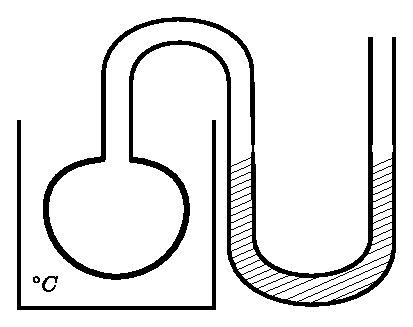
\includegraphics[width=\textwidth]{termo_1/termo_1_5}
            \newsubcap{Gay-Lussac I. törvényének mérési elrendezése}
            %\phantomsubcaption
            \label{fig:termo_1_5}
    \end{subfigure}
    \phantomcaption
    \end{figure}
    \item \emph{Gay-Lussac II.~törvénye:} Állandó térfogaton melegítés hatására nő a gáz nyomása. A hőmérséklet és a nyomás között egyenes arányosság áll fent. Igaz, hogy:
    \begin{align}
        p(t) = p_0(1+\beta t),
    \end{align}
    ahol $p$ a nyomás, $p_0$ pedig a $0\,^\circ$C-on mért nyomás. Fontos megállapítás, hogy a Gay-Lussac I.~és II.~törvényében megjelenő $\beta$ ugyanaz, értéke pedig a kísérletek alapján $\beta = 1/273{,}16\, ^\circ\mathrm C$. Ez igaz minden ideális gázra (a hélium például nagyon jó közelítéssel ideális gáznak tekinthető).
\end{itemize}
Ezek alapján az ideális gáz állapotegyenletét már meghatározhatjuk az alábbi gondolatkísérlettel. Induljunk ki egy $0\,^\circ\text C$-os ideális gázból, melynek térfogata $V_0$, nyomása pedig $p_0$. Először állandó nyomáson növeljük meg a hőmérsékletét $t$-re, majd állandó hőmérsékleten a térfogatát változtassuk $V$-re. Így tetszőleges $t$ és $V$ elérhető. A folyamatot lásd \aref{fig:termo_1_2}. ábrán.
A fenti törvények alapján ekkor:
\begin{align}
    \begin{array}{rcl} V_1\hspace{-2mm} &=& \hspace{-2mm}V_0(1+\beta t)\\ \quad p_0V_1 \hspace{-2mm}&=&\hspace{-2mm} pV\end{array}  \quad\Rightarrow\quad pV = p_0V_0(1+\beta t)=\underbrace{p_0V_0\beta}_{\substack{=nR,\\\textnormal{ez mérhető}}}\hspace{-2mm} T\quad\Rightarrow\quad pV = nRT,
\end{align}
ahol $T = t+1/\beta$ a Kelvinben mért hőmérséklet, $n$ jelöli az anyagmennyiséget\footnote{\,A mértékegysége $[n] = \textnormal{mol}$, 1 mol a 12 g $^{12}$C-ben lévő atomok száma.}, $R=8{,}314 \text{ J}/\left(\text{mol K}\right)$ az univerzális gázállandó. Az $n$ anyagmennyiség meghatározható egyrészt az Avogadro\footnote{\,Amadeo Avogadro, 1776-1856.}-állandó ($N_A \approx 6\cdot 10^{23}$) segítségével és az összes részecske számával mint $n = N/N_A$, illetve ha ismert a teljes rendszer tömege ($m$), illetve a moláris tömeg ($M$), akkor $n = m/M$. \Aref{fig:termo_1_3}. ábrán látható, hogy tényleg Kelvin-skálára áttérve 0K-en lesz a gáz térfogata zérus.
\begin{figure}[!h]
    \centering
    \begin{subfigure}[t]{0.45\textwidth}
            \centering
            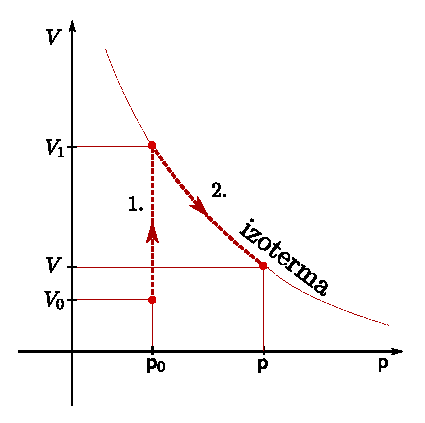
\includegraphics[width=\textwidth]{termo_1/termo_1_2}
            \newsubcap{Folyamat a $\pres-V$ síkon, melyből az állapotegyenlet meghatározható.}
            \label{fig:termo_1_2}
    \end{subfigure}\hfill
    \begin{subfigure}[t]{0.45\textwidth}
            \centering
            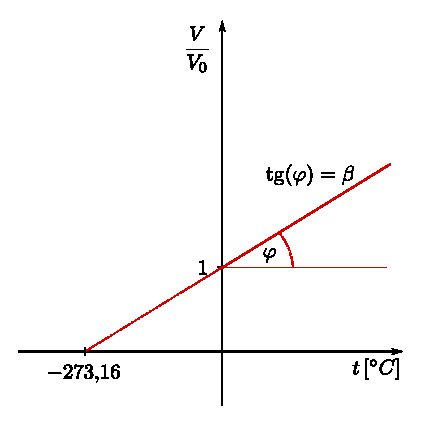
\includegraphics[width=\textwidth]{termo_1/termo_1_3}
            \newsubcap{Kelvin-skálára áttérve 0K-en lesz a gáz térfogata zérus, az egyenes meredeksége pedig pont $\beta$.}
            \label{fig:termo_1_3}
    \end{subfigure}
    \end{figure}
Az előzőek alapján az ideális gáz állapotegyenlete tehát:
\begin{align}
    pV = nRT.
\end{align}
\section{Anyagi tulajdonságok}

\emph{Hőtágulás: lineáris és térfogati; Különleges viselkedésű anyagok; Kompresszibilitás; Feszültségi együttható; Hármasszabály; Összefüggés az anyagi paraméterek között; Ideális gáz anyagi tulajdonságai.}

Kísérleti tapasztalat, hogy ha fémrudat melegítünk, akkor annak a hossza megnő. Sőt általánosan is igaz, hogy hőmérsékletváltozás hatására a testek hossza, térfogata megváltozik. Sok esetben a hőmérséklet és a hossz között lineáris kapcsolat áll fent, ahol az \aref{fig:termo_2_1}. ábrán is látható:
\begin{align}
    l = l_0(1+\alpha' T),
\end{align}
ahol $\alpha'$ a \emph{lineáris hőtágulási együttható}. Némely esetben azonban a hossz és  a hőmérséklet között teljesen bonyolult kapcsolat is lehet\footnote{\,Gondoljunk csak például a vízre, melynek a sűrűsége 4$^\circ$C körül a legnagyobb, ezért szoktak elfagyni a vízvezetékek, ha nem zárják el azt télre. Másik érdekes anyag a gumi. Kipróbálhatjuk, hogy befőttesgumit berakunk a fagyasztóba. Azt fogjuk tapasztalni, hogy a fagyasztóból kivett befőttesgumi összemegy.}, ekkor az $l(T)$ görbe érintőjét tudjuk csak meghatározni, ahogy az \aref{fig:termo_2_2}. ábrán is látható.
\begin{figure}[!h]
    \centering
    \begin{subfigure}[t]{0.45\textwidth}
            \centering
            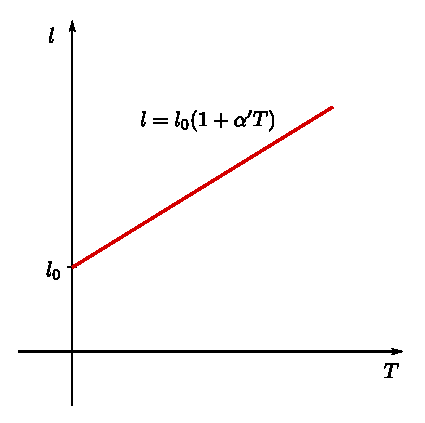
\includegraphics[width=\textwidth]{termo_2/termo_2_1}
            \newsubcap{Hőtágulás lineáris hőtágulási együtthatóval.}
            \label{fig:termo_2_1}
    \end{subfigure}\hfill
    \begin{subfigure}[t]{0.45\textwidth}
            \centering
            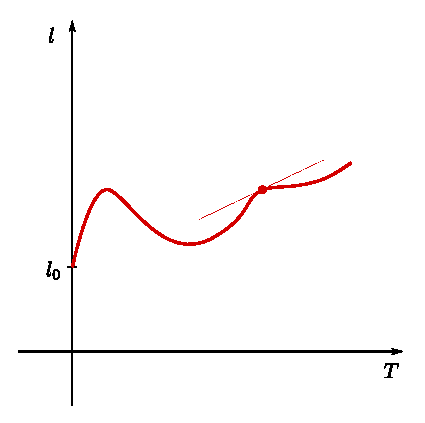
\includegraphics[width=\textwidth]{termo_2/termo_2_2}
            \newsubcap{Hőtágulás bonyolult alakú hőtágulási együtthatóval, amikor csak az adott hőmérséklethez tartozó érintőből határozható meg a hőtágulási együttható.}
            \label{fig:termo_2_2}
    \end{subfigure}
    \end{figure}
Az állandó nyomáson vett lineáris hőtágulási együttható általános esetben definíció szerint:
\begin{align}
    \alpha = \rec l \pd{l}{T}\bigg|_\pres,
\end{align}
ami tehát megadja, hogy állandó nyomáson a test hőmérsékletét változtatva mennyivel változik meg annak a hossza. Az $1/l$ azért van beledefiniálva, hogy a test hosszától független, csak az anyagi minőségtől függő mennyiséget kapjunk. A definíció szerint $[\alpha]~{=}~\frac 1K$, értéke pedig szilárd testekre $\alpha_{\tn{szilárd}}~{\sim}~10^{-5} \frac 1K$, míg folyadékokra $\alpha_{\tn{folyadék}}~{\sim}~10^{-4} \frac 1K$. Érdemes észrevenni, hogy általában $\alpha\neq\alpha'$, hiszen a $\alpha$ esetében mindig az aktuális hosszal osztunk le:
\begin{align}
    l(T) = l_0(1+\alpha' T)\Rightarrow \Delta l = l_0\alpha' T \Rightarrow \alpha = \rec l \pd{l}{T}\bigg|_\pres = \rec{l_0(1+\alpha' T)}l_0\alpha' = \frac{\alpha'}{1+\alpha' T}.
\end{align}
Ha a hőtágulási együttható negatív az azt jelenti, hogy az anyag a hőmérséklet növelésével összemegy, ilyen például a víz 0$^\circ$C és 4$^\circ$C között, a gumiszál, a damil, a vasdrót 1000$^\circ$C-on illetve a szilícium 18K-120K között.

Hőmérsékletváltozás hatására nem csak az anyagok hossza, hanem a térfogata is megváltozik. Egy $l$ oldalú kocka térfogatváltozása:
\begin{align}
\begin{split}
    V &= l^3 = \big(l_0(1+\alpha' T) \big)^3 = \underbrace{l_0^3}_{=V_0}(1+3\alpha' T +3{\alpha'}^2 T^2 + {\alpha'}^3 T^3) =\\
    &=V_0(1+\underbrace{3\alpha'}_{\beta'} T) + \mathcal O({\alpha'}^2) \approx V_0(1+\beta' T),
\end{split}
\end{align}
ahol felhasználtuk hogy $\alpha'$ másodrendűen kicsi\footnote{\,Ezt jelöltük a ,,nagy ordó'' szimbólummal, $\mathcal O$, az argumentumában szereplő mennyiségekkel, illetve azok magasabb rendű hatványai elhanyagolhatóak.}, így csak a lineáris rendig mentünk el. Bevezettük a $\beta' = 3\alpha'$ \emph{térfogati hőtágulási együtthatót} is, mely általános esetben állandó nyomáson definíció szerint:
\begin{align}
    \beta = \rec V \pd{V}{T}\bigg|_\pres,
\end{align}
ahol az $1/V$ újfent azért kellett, hogy csak az anyagi minőségtől függő állandót kapjunk, továbbá $\beta\neq\beta'$. Állandó nyomáson vett lineáris térfogati hőtágulási együtthatóra láthatunk néhány példát \aref{fig:termo_2_3}. ábrán. Ideális gáz esetében:
\begin{align}
    V = \frac{nRT}{\pres} \follows \pd{V}{T}\bigg|_\pres = \frac{nR}{\pres} \follows \beta_{\tn{id.g.}} = \frac{nR}{\pres V}=\rec T,
\end{align}
ami $T = 273{,}16$K esetén megegyezik az ideális gáz esetén bevezetett $\beta'$-vel ($\beta' = \rec{273{,}16K}$, $\beta=\beta'(T{=}273{,}16K$)). A hőmérsékletet mindenhol K-ben értjük. Láthatjuk tehát, hogy az ideális gáznak lineáris a hőtágulása.

A folytonos közegek mechanikájának tárgyalása során is találkoztunk már a \emph{kompresszibilitás} fogalmával, ami állandó hőmérsékleten definíció szerint:
\begin{align}
    \kappa = -\rec V \pd{V}{\pres}\bigg|_T,
\end{align}
ahol a negatív előjel azért szerepel a definícióban, mert a derivált minden esetben negatív kell legyen, hiszen különben a rendszer instabil lenne (külső nyomás hatására kitágulna). \Aref{fig:termo_2_4}. ábrán látható néhány példa állandó hőmérsékleten vett kompresszibilitásra, ha az összefüggés lineáris. 
\begin{figure}[!h]
    \centering
    \begin{subfigure}[b]{0.48\textwidth}
            \centering
            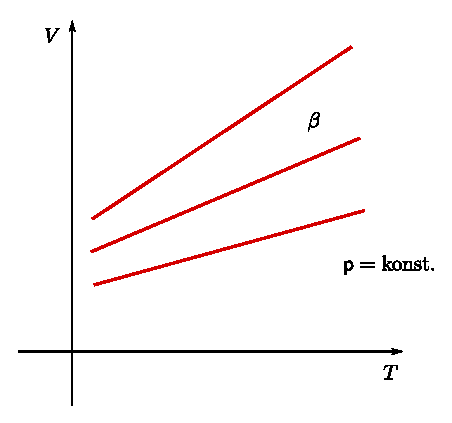
\includegraphics[width=\textwidth]{termo_2/termo_2_3}
            \newsubcap{Térfogati hőtágulás lineáris hőtágulási együtthatóval.}
            \label{fig:termo_2_3}
    \end{subfigure}\hfill
    \begin{subfigure}[b]{0.45\textwidth}
            \centering
            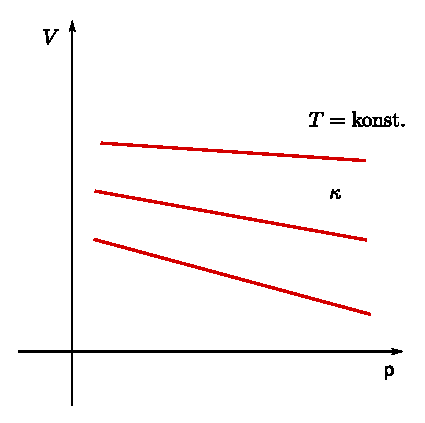
\includegraphics[width=\textwidth]{termo_2/termo_2_4}
            \newsubcap{Izoterm kompresszibilitás lineáris esetben.}
            \label{fig:termo_2_4}
    \end{subfigure}
    \end{figure}
Ideális gáz esetén:
\begin{align}
    V = \frac{nRT}{\pres} \follows \kappa_{\tn{id.g.}} = -\rec V \pd{V}{\pres}\bigg|_T = -\rec V \z{-\frac{nRT}{\pres^2}}= \rec \pres.
\end{align}
Definiálhatjuk még a \emph{feszültségi együtthatót} is állandó térfogaton a következőképp:
\begin{align}
    \gamma = \rec \pres \pd{\pres}{T}\bigg|_V,
\end{align}
mely ideális gázra:
\begin{align}
    \gamma_{\tn{id.g.}} = \rec \pres\frac{nR}{V} = \rec T.
\end{align}
A feszültségi együttható azt fejezi ki, hogy ha állandó térfogaton melegítünk egy rudat, majd lehűtjük, akkor benne feszültség keletkezik\footnote{\,Érdemes utánanézni a bolognai üvegcseppnek.}.
Mivel $\beta$, $\kappa$ és $\gamma$ definíciói meglehetősen hasonlóak, gondolhatjuk, hogy valamilyen kapcsolat áll fent ezen mérhető mennyiségek között, nem függetlenek egymástól. Induljunk ki abból, hogy az állapotegyenlet egy $f(\pres,V,T)=0$ függvény, ami egy 3d-s felületet határoz meg, lásd \aref{fig:termo_2_5}. ábrán. Ideális gáz esetében ez az összefüggés ugye $\pres V-nRT=0$. Ideiglenesen bevezetjük az alábbi jelöléseket:
\begin{align}
    \pres = \mathsf P(v,t),\quad v=V(\pres,t),\quad t=T(\pres,v).
\end{align}
Itt $\mathsf P$,$V$ és $T$ jelöli a függvényeket, $\pres$,$v$ és $t$ pedig a függvényérték. Számítsuk ki az alábbi deriváltat:
\begin{align}\label{eq:harmas_1}
    \pd{}{v}v = \pd{}{v}V(\mathsf P(v,t),t)\follows 1 = \pd V\pres\bigg|_t\cdot \pd{\mathsf P}{v}\bigg|_t.
\end{align}
Deriváljunk most $t$ szerint:
\begin{align}\label{eq:harmas_2}
    \pd{}{t}v = \pd{}{t}V(\mathsf P(v,t),t) \Rightarrow 0 = \pd{V}{\pres}\bigg|_t\cdot \pd{\mathsf P}{t}\bigg|_v+\pd{V}{t}\bigg|_\pres \Rightarrow \pd{V}{\pres}\bigg|_t\cdot \pd{\mathsf P}{t}\bigg|_v = -\pd{V}{t}\bigg|_\pres.
\end{align}
A (\ref{eq:harmas_1})-(\ref{eq:harmas_2}). egyenleteket összevonva és visszatérve a szokásos $\pres$,$V$,$T$ jelölésekre kapjuk, hogy:
\begin{align}
    \pd{V}{\pres}\bigg|_T\cdot \pd{\pres}{T}\bigg|_V\cdot \pd{T}{V}\bigg|_\pres = -1 \follows (-V\kappa)\cdot(\pres\gamma)\cdot\z{\rec{\beta V}} = -1 \follows \frac{\pres\kappa \gamma}{\beta} = 1,
\end{align}
ami igaz minden anyagra (behelyettesítéssel leellenőrizhetjük például az ideális gázra kiszámolt mennyiségekre is). A
\begin{align}
    \pd{V}{\pres}\bigg|_T\cdot \pd{\pres}{T}\bigg|_V\cdot \pd{T}{V}\bigg|_\pres = -1
\end{align}
összefüggést szokás \emph{hármasszabálynak} hívni.

Tekintsünk most egy általános $f(x,y)$ kétváltozós függvényt, lásd \aref{fig:termo_2_6}. ábrát.
\begin{figure}[!h]
    \centering
    \begin{subfigure}[]{0.45\textwidth}
            \centering
            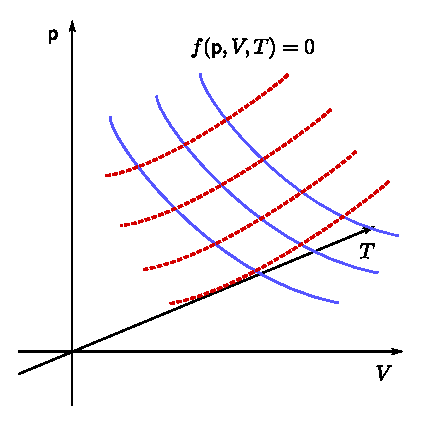
\includegraphics[width=\textwidth]{termo_2/termo_2_5}
            \newsubcap{$f(\pres,V,T)=0$ függvény, ami egy 3d-s felületet határoz meg a térben.}
            \label{fig:termo_2_5}
    \end{subfigure}\hfill
    \begin{subfigure}[]{0.45\textwidth}
            \centering
            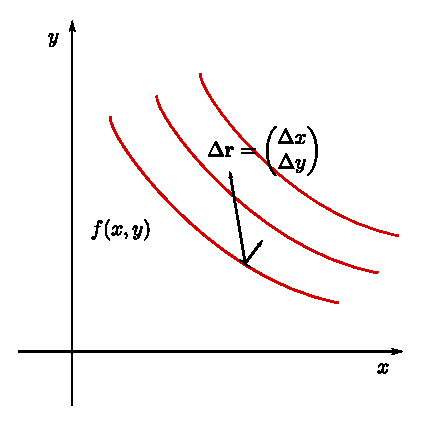
\includegraphics[width=\textwidth]{termo_2/termo_2_6}
            \newsubcap{Példa egy $f(x,y)$ kétváltozós függvény megváltozására.}
            \label{fig:termo_2_6}
    \end{subfigure}
\end{figure}
Ekkor az $f(x{+}\Delta x{,}y{+}\Delta y)$ kifejezést Taylor-sorba fejthetjük:
\begin{align}
    f(x{+}\Delta x,y{+}\Delta y)\approx f(x,y) + \bm\nabla f \Delta \bm r{+}\mathcal O(\Delta \bm r^2),\quad \tn{ahol}\quad \bm\nabla f \Delta \bm r = \pd fx\Delta x+\pd fy \Delta y.
\end{align}
A függvény megváltozása tehát elsőrendben:
\begin{align}
    \Delta f\approx \pd fx\Delta x+\pd fy \Delta y \follows \m df = \pd fx\bigg|_y\m d x+\pd fy\bigg|_x \m d y.
\end{align}
Ezutóbbit a függvény \emph{teljes deriváltjának} nevezzük. Alkalmazva ezt a $V(\pres,T)$ és $\pres(V,T)$ függvényekre kapjuk, hogy:
\begin{align}
    \m d V &= \pd V\pres\bigg|_T \m d\pres + \pd VT\bigg|_\pres \m dT \\
    \m d \pres &= \pd{\pres}{V}\bigg|_T\m dV + \pd{\pres}{T}\bigg|_V \m dT = \frac{1}{\pd{V}{\pres}\big|_T}\,\m d V - \frac{\pd{V}{T}\big|_\pres}{\pd{V}{\pres}\big|_T}\,\m d T,
\end{align}
ahol az utóbbi egyenlőségnél alkalmaztuk a hármasszabályt.

\section{Kinetikus gázelmélet}

\emph{Feltevések; Ideális gáz állapotegyenletének származtatása; Hőmérséklet értelmezése; Ekvipartíció; Szabadsági fokok száma és hőmérsékletfüggése.}

Megismerkedtünk már korábban az ideális gázzal, ami például hélium esetén jó közelítéssel leírja a valódi gáz viselkedését. A valódi gázok leírásával a továbbiakban fogunk még részletesen foglalkozni, azonban először az ideális gázok egyszerű modelljével, a \emph{kinetikus gázelmélettel} ismerkedünk meg. Bernoulli\footnote{Daniel Bernoulli, 1700-1782. Ő ugyanaz a Bernoulli, aki a hidrodinamika Bernoulli-törvényét is kitalálta, azonban egyébként számos híres Bernoulli volt a családban, akik a fizika és a matematika szerteágazó területén tevékenykedtek.} ötlete volt 1738-ban a kinetikus gázelmélet, miszerint tegyük fel, hogy (ennek egy részével már találkoztunk az ideális gázok kapcsán):
\begin{itemize}
    \item a vizsgálandó gázt bezárjuk egy az $x$,$y$,$z$ tengelyek irányával egybeeső kockába, melynek térfogata $V$, az összes részecske száma $N$,
    \item a gázt alkotó atomok vagy molekulák térfogata a gáz által kitöltött térfogathoz képest elhanyagolható, a részecskék pontszerűek, a tömegük legyen $\mu$.
    \item a gázmolekulák egymással ütköznek, azonban más (taszító vagy vonzó) kölcsönhatásban egymással nem állnak,
    \item a gázmolekulák egymással illetve a fallal vett ütközése tökéletesen rugalmas,
    \item mindegyik részecske $v$ sebességgel mozog vagy az $x$,$y$ vagy $z$ tengely irányába, és mindegyik irányba ugyanannyi részecske halad,
    \item a részecskék egyenletesen töltik ki a teret (homogén rendszer, nincs köztük korreláció).
\end{itemize}
Az összeállítás látható \aref{fig:termo_3_1}. ábrán.
\begin{figure}
    \centering
    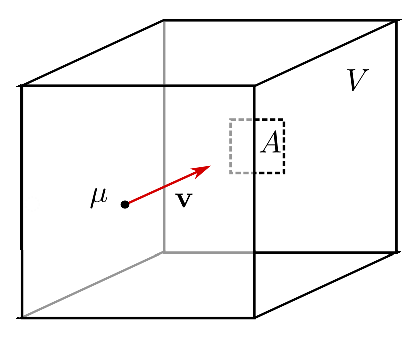
\includegraphics{termo_3/termo_3_1.eps}
    \caption{Ideális gáz kinetikus modellje.}
    \label{fig:termo_3_1}
\end{figure}
Ezen egyszerű feltevések alapján fogjuk meghatározni a rendszer kinetikus energiáját. Bevezetünk néhány jelölést, amit a továbbiakban is használni fogunk\footnote{\,A legtöbb könyv és jegyzet ugyanazt a $p$ betűt használja a nyomásra, impulzusra és a valószínűségre is, az ebből eredő esetleges félreértéseket igyekszünk kikerülni.}. Az impulzust $\mom$, a nagyságát pedig $|\mom|\equiv p$ jelöli. ``Talpas'' $\prob$ jelöli a valószínűséget, a nyomásra pedig $\pres$ betűvel hivatkozunk. Ismert összefüggések a nyomásra és az erőre, hogy:
\begin{align}
    \pres = \frac FA,\qquad \bm F = \md \mom t.
\end{align}
Vizsgáljunk most a ${+}x$ tengely irányába haladó részecskéket, melyek száma értelemszerűen a feltevéseink alapján $N/6$. Rugalmasan ütköznek a kocka falán, általuk a falra kifejtett nyomás:
\begin{align}
    \pres = \frac{F_x}{A} = \frac{\Delta p_x}{A\cdot \Delta t} = \frac{\frac N6 \mu \cdot \Delta v_x}{A\cdot \Delta t} = \frac{\frac N6 \mu\cdot 2v}{A\cdot \Delta t} = \rec{6A\cdot\Delta t}\frac NV \underbrace{Av\Delta t}_{\equiv V}\cdot 2\mu v = \frac 13 \frac NV \mu v^2.
\end{align}
Ezt kicsit átalakítva kapjuk, hogy:
\begin{align}
    pV = \frac 23 \underbrace{N\frac 12\mu v^2}_{\equiv E_{\tn{kin}}} = \frac 23 E_{\tn{kin}} = nRT,
\end{align}
ahol az utolsó egyenlőségjelnél felhasználtuk az ideális gáz állapotegyenletét. Ebből egyszerű átalakításokkal és a korábban tanult mennyiségekkel adódnak az alábbi relációk:
\begin{align}
    E_{\tn{kin}} = \frac 32 nRT = \frac 32 \frac{N}{N_A} RT = N\frac 12 \mu v^2 \follows \frac 32 \underbrace{\frac{R}{N_A}}_{\equiv k_B} T = \frac 12 \mu v^2,
\end{align}
ahol bevezettük a Boltzmann\footnote{\,Ludwig Boltzmann, 1844-1906.}-állandót, $k_B = R/N_A = 1{,}38\cdot 10^{-23} \tn{J/K}$. Így tehát a gázrészecskék átlagos sebességével, energiájával a hőmérséklet kifejezhető, hiszen egy részecske kinetikus energiája:
\begin{align}\label{eq:ekv_part}
    E_{\tn{1,kin}} = \frac 32 k_B T = \frac 12 \mu v^2 = \frac 12\mu \big(\langle v_x^2 \rangle + \langle v_y^2 \rangle + \langle v_z^2 \rangle\big),
\end{align}
ahol $\langle . \rangle$ egy mennyiség várható értékét\footnote{\,Egy kis valószínűségszámítási ismétlés: diszkrét esetben legyenek egy $x$ mennyiség lehetséges értékei $x_1,x_2,\dots x_N$ rendre $\prob_1,\prob_1,\dots \prob_N$ valószínűséggel. Ekkor az $x$ mennyiség várható értékének nevezzük az $\langle x \rangle = \sum\limits_{i=1}^N \prob_i x_i$ kifejezést ($\sum\limits_{i=1}^N \prob_i = 1$ a mellékfeltétel). Folytonos valószínűségi változónál jelölje $\rho(x)$ a sűrűségfüggvényt ($\int\limits_{-\infty}^\infty \rho(x) \m d x = 1$). Ekkor a várható érték a következő: $\langle x \rangle = \int\limits_{-\infty}^\infty \rho(x)x \m d x$. Hasonlóan értelmezhető például, hogy $\langle x^n \rangle = \int\limits_{-\infty}^\infty \rho(x)x^n \m d x$ tetszőleges $n\in \mathbb N$ számra. Fontos megjegyezni, hogy $\langle x^2\rangle \neq \langle x \rangle ^2$, sőt pont ezeknek a különbsége a szórásnégyzet: $\sigma^2 = \langle (x - \langle x \rangle)^2 \rangle =  \langle x^2\rangle - \langle x \rangle ^2$. Felhasználtuk továbbá a (\ref{eq:ekv_part}). összefüggésben, hogy a határozott integrál integrandusának additivitásából következik, hogy $\langle x_1+x_2 \rangle = \langle x_1 \rangle + \langle x_2 \rangle$.} jelöli. Hélium esetében $300$K-en $\sqrt{\langle v^2 \rangle} \sim 10^4 m/s$. Láthattuk, hogy a rendszer teljes kinetikus energiája $\frac 32 k_BT$. A részecskék a koordináta-rendszer három tengelye ($x$,$y$,$z$) irányába is mozoghatnak, továbbá mivel a sebességnégyzetek várható értéke a három koordinátatengely irányába megegyezik termikus egyensúly esetében, ezért azt mondhatjuk, hogy mindegyik kvandratikus energiatagnak a várható értéke $\frac 12 k_BT$, ezt hívjuk az \emph{ekvipartíció tételének}. Bevezetjük a \emph{szabadsági fokok} számát, amit $f$-fel jelölünk, ez fejezi ki, hogy ,,hány kvadratikus tag van''. Egyatomos ideális gázra $f=3$, kétatomos gázra\footnote{\,Itt már két forgási irányt is meg lehet különböztetni.} $f=5$, többatomos gázra illetve szilárdtestekre\footnote{\,A szilárdtestek atomjai is hőmozgást végeznek, amit modellezhetünk úgy, mint egymáshoz $D$ rugóállandójú rugóval csatolt atomok, ahogy az \aref{fig:termo_3_2}. ábrán is látható. Ez is 3 kvadratikus energiatagot jelenít meg ($\frac 12 D(x^2+y^2+z^2)$), azaz a szabadsági fokok száma: $3 \tn{ mozgási} + 3 \tn{ rugalmas} = 6$.} $f=6$.
\begin{figure}
    \centering
    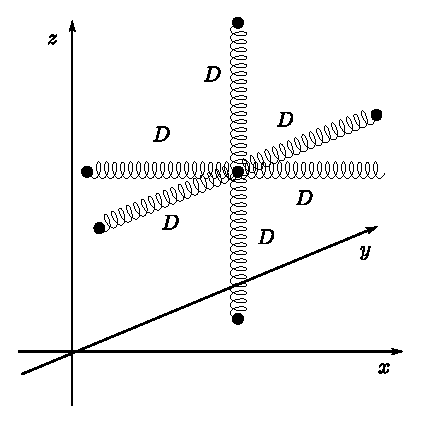
\includegraphics{termo_3/termo_3_2.eps}
    \caption{Szilárdtestek rezgésének modellezése $D$ rugóállandójú rugókkal.}
    \label{fig:termo_3_2}
\end{figure}
A szabadsági fokokkal kifejezve a rendszer kinetikus energiája:
\begin{align}
    E_{\tn{kin}} = \frac f2 Nk_B T.
\end{align}
Általános esetben a dobozba zárt részecskék sebessége nem azonos, hanem az ún. \emph{Maxwell\footnote{\,James Cleck Maxwell, 1831-1879.}--Boltzmann-eloszlást} követik, a részecskék sebességének eloszlása nagyban függ a hőmérséklettől. A Maxwell--Boltzmann-eloszlással később még részletesen fogunk foglalkozni, ezért itt mélyebben nem tárgyaljuk.
\section{Reális gázok}

\emph{Feltevések; van der Waals állapotegyenlet levezetése; a és b paraméterek jelentése; Kritikus pont; Állapotegyenlet redukált alakja}

Mindeddig ideális gázokkal foglalkoztunk, melyek azokban egy túlságosan leegyszerűsített modelljét alkotják a valódi gázoknak. Reális gázoknál a részecskéknek véges a méretük, illetve köztük kölcsönhatás van. A kölcsönhatást leggyakrabban az ún. Lennard-Jones\footnote{\,John Lennard-Jones, 1894-1954.}-potenciállal szokás figyelembe venni\footnote{\,A potenciál alakja nagyrészt empirikus: a részecskék között ún. Van der Waals-féle vonzó kölcsönhatás van, azonban amikor túl közel kerülnek egymáshoz, akkor taszításnak kell fellépnie (azért, hogy ,,ne ütközzenek egymásnak''). Az $r^{-6}$ tag az ún. indukált polarizáció következménye, az $r^{-12}$-tagnak viszont konkrét fizikai tartalma nincs, számítási szempontból praktikus ($r^{-6}$-t kell csak négyzetre emelni). A $\varepsilon$ és $\sigma$ paraméterek anyagi állandók. Vannak a Lennard-Jones-modellen túlmutató potenciálok is, amelyek például nem párkölcsönatáson alapulnak, de ezekkel most nem foglalkozunk.}:
\begin{align}
    U_{\tn{L-J}} = 4\varepsilon\z{\z{\frac{\sigma}{r}}^{12}-\z{\frac{\sigma}{r}}^6}.
\end{align} 
A Lennard--Jones-potenciál alakját láthatjuk \aref{fig:termo_4_4}. ábrán. Ideális gáznál a $\pres-V$ diagramon hiperbolák voltak az állapotegyenlet miatt ($\pres\propto \rec V$; ld. \ref{fig:termo_4_1}. ábra). Itt a részecskék véges kiterjedése következtében van egy minimális térfogat, nem lehet végtelen kicsire összenyomni a gázt (ld. \ref{fig:termo_4_2}. ábra); a minimális térfogat:
\begin{align}
    V_{\tn{min}} = nb,
\end{align}
ahol $n$ az anyagmennyiség, $b$ pedig anyagi állandó.
\begin{figure}[!h]
    \centering
    \begin{subfigure}[t]{0.45\textwidth}
            \centering
            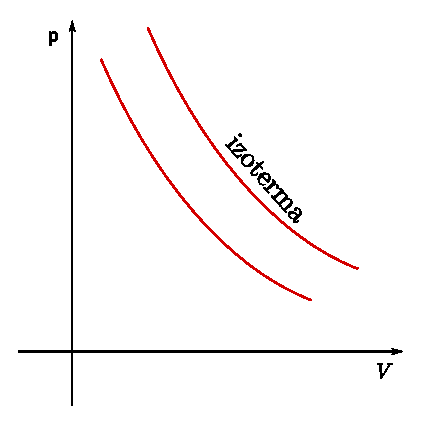
\includegraphics[width=\textwidth]{termo_4/termo_4_1}
            \newsubcap{Ideális gáznál az izotermák hiperbolák.}
            \label{fig:termo_4_1}
    \end{subfigure}\hfill
    \begin{subfigure}[t]{0.45\textwidth}
            \centering
            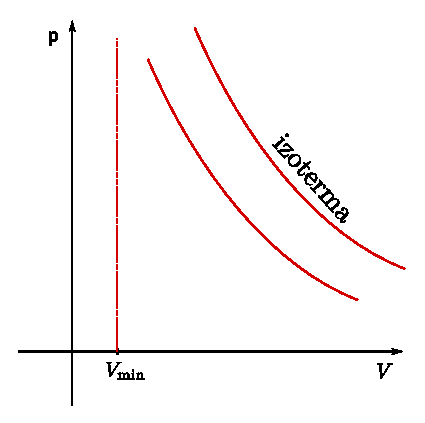
\includegraphics[width=\textwidth]{termo_4/termo_4_2}
            \newsubcap{Reális gázoknál van egy minimális térfogat, aminél kisebbre nem lehet összenyomni a gázt.}
            \label{fig:termo_4_2}
    \end{subfigure}
\end{figure}
Az ideális gáz állapotegyenlete emiatt már mindenképp javításra szorul:
\begin{align}\label{eq:vdW_1}
    \pres(V-nb) = nRT \follows \pres = \frac{nRT}{V-nb},
\end{align}
azonban nem vettük még figyelembe a kölcsönhatás járulékát. Mivel a van der Waals\footnote{\,Johannes Diderik van der Waals, 1837-1923.}-kölcsönhatás csak nagyon rövid távolságon taszító, egyébként pedig vonzó (de így is gyorsan lecsengő), ezért összességében kisebb nyomást fognak kifejteni a részecskék a doboz falának ütközve, ahogy ezt a \ref{fig:termo_4_3}. ábrán is szemléltetjük.
\begin{figure}
    \centering
    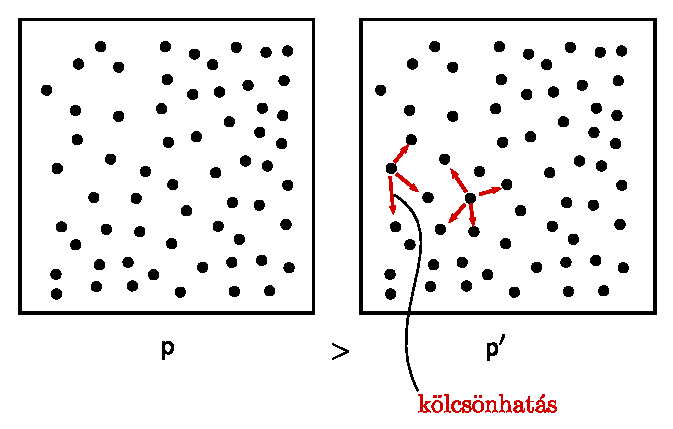
\includegraphics{termo_4/termo_4_3.eps}
    \caption{Van der Waals-gázoknál a nyomás csökken a részecskék vonzó kölcsönhatása miatt. Bal oldalon a kölcsönhatásmentes esetet látjuk, jobb oldalon pedig pár gázmolekulára berajzoltunk néhány rá ható erőt, ezt jelölik a piros nyilak.}
    \label{fig:termo_4_3}
\end{figure}
Igyekezzünk ezt megbecsülni! Ehhez tekintsünk egy egyszerűsített modellt, ahol a rövid távú kölcsönhatást egy konstans $-F_0$ erővel vesszük figyelembe $d$ távolságig (ld. \ref{fig:termo_4_5}. ábra), azaz:
\begin{align}
    F =
    \begin{cases}
    F_0<0,&\tn{ha}\quad r<d\\
    0,&\tn{egyébként}.
    \end{cases}
\end{align}
\begin{figure}[!h]
    \centering
    \begin{subfigure}[t]{0.45\textwidth}
            \centering
            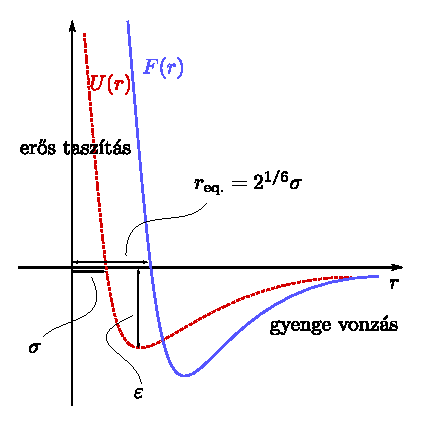
\includegraphics[width=\textwidth]{termo_4/termo_4_4}
            \newsubcap{Lennard--Jones-potenciál.}
            \label{fig:termo_4_4}
    \end{subfigure}\hfill
    \begin{subfigure}[t]{0.45\textwidth}
            \centering
            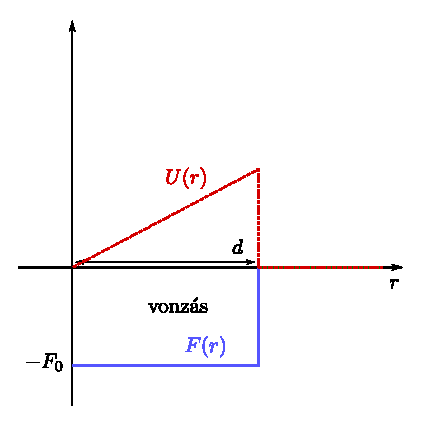
\includegraphics[width=\textwidth]{termo_4/termo_4_5}
            \newsubcap{A Lennard--Jones-potenciáls leegyszerűsített modellje konstans $-F_0$ erővel $d$ távolságig.}
            \label{fig:termo_4_5}
    \end{subfigure}
\end{figure}
Hogyan változik meg a nyomás ennek a kölcsönhatásnak a következtében? Egy gázrészecske annak $d$ sugarú környezetében $N_{\tn{pár}}$ számú részecskével hat kölcsön (ld. \ref{fig:termo_4_6}. ábra):
\begin{align}
    N_{\tn{pár}} \approx \overbrace{\rho\underbrace{Ad}_{=V}}^{\substack{\tn{részecskék}\\\tn{száma}}}\cdot\overbrace{\rho d^3}^{\substack{\tn{1 részecskére}\\\tn{jutó $d$}\\\tn{sugarú gömb}}},\quad \tn{ahol }\rho=\frac NV\tn{ a részecskesűrűség}.
\end{align}
\begin{figure}
    \centering
    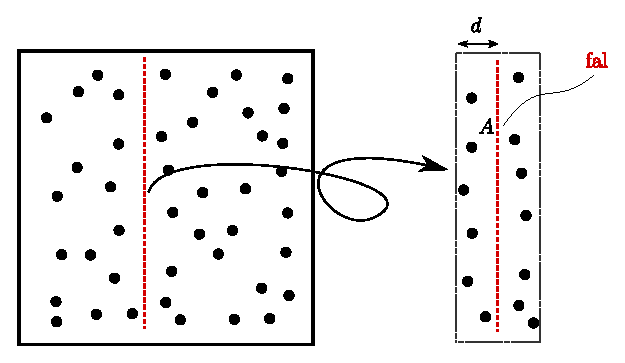
\includegraphics{termo_4/termo_4_6.eps}
    \caption{Rövid távú kölcsönhatás, mely a gázrészecskék $d$ sugarú környezetében hat.}
    \label{fig:termo_4_6}
\end{figure}
Ezekkel a teljes nyomás megváltozása:
\begin{align}
    \Delta\pres = \frac{F_{\tn{össz}}}{A}\sim \frac{F_0N_{\tn{pár}}}{A}\sim \frac{F_0}{A}\rho^2 A d^4 = F_0d^4\z{\frac nV}^2 = -a\z{\frac nV}^2,
\end{align}
ahol $a$ anyagi állandó, a negatív előjel pedig azért jelenik meg, mert a nyomás csökken a kölcsönhatásnak köszönhetően. A (\ref{eq:vdW_1}). egyenletet továbbírva kapjuk, hogy:
\begin{align}
    \pres = \frac{nRT}{V-nb}-a\z{\frac nV}^2 \follows \sz{\pres+a\z{\frac nV}^2}(V-nb) = nRT,
\end{align}
ez a \emph{van der Waals-gáz állapotegyenlete}, van der Waals érte Nobel-díjat kapott 1910-ben\footnote{\,Az állapotegyenlet kölcsönható rendszerek statisztikus fizikai számolásával is meghatározható, ugyanerre az eredményre jutunk elsőrendben.}. Az állapotegyenlet görbéi a $\pres-V$ síkon már nem hiperbolák, hanem bonyolult harmadfokú kifejezések. Kiszámolható az izoterm kompresszibilitás\footnote{\,Nem kell tudni, de $$\kappa_{vdW} = -\rec V \rec{\frac{2an^2}{V^3}-\frac{nRT}{(V-nb)^2}}$$.}, ami egy adott tartományon negatív is lehet, így ott a gáz instabillá válna, tehát ez egy tiltott tartomány, az izotermák (azonos hőmérsékletű görbe) ezt a tartományt ,,átugorják''. Keressük meg a kritikus pontot, ahol az $\pres-V$ grafikon egy izotermájának inflexiós pontja van, ahogy ez \aref{fig:termo_4_7}. ábrán is látható.
\begin{figure}
    \centering
    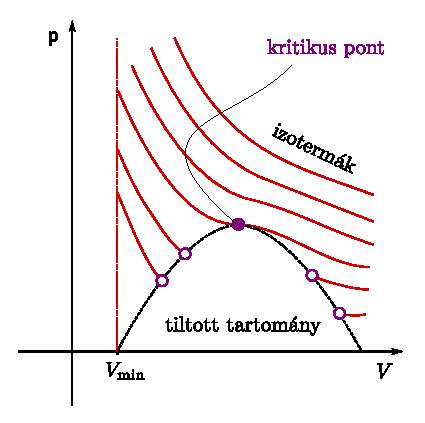
\includegraphics{termo_4/termo_4_7.eps}
    \caption{Van der Waals-gáz a $\pres-V$ diagramon. Látható rajta a kritikus pont, illetve a tiltott tartomány.}
    \label{fig:termo_4_7}
\end{figure}
A kritikus pont alatt a nyomásnak ugrása van, ami másodrendű (folytonos) fázisátalakulást jelent (a fáziátalakulásokról még részletesen szó fog esni a kurzus hátralévő részén). A kritikus pont értékeire adódik\footnote{\,Egyrészt a kompresszibilitás feltételéből adódik (ami ekvivalens a $\pd \pres V\big|_{T=T_c}=0$ feltétellel; itt $T_c$ a kritikus pont hőmérséklete): $$ \frac{2an^2}{V_c^3}-\frac{nRT_c}{(V_c-nb)^2}=0,$$
másrészt a $$\frac{\partial^2\pres}{\partial V^2}\bigg|_{T=T_c}=0$$ feltételből kapjuk, hogy:
$$\frac{2nRT_c}{(V_c-bn)^3}-\frac{6an^2}{V_c^4}=0.$$ Ebből a két egyenletből a kritikus pont paraméterei meghatározhatóak.}, hogy:
\begin{align}
    V_c = 3bn,\quad p_c = \frac{8}{27}\frac{a}{Rb},\quad T_c = \frac{1}{27}\frac{a}{b^2}.
\end{align}
\Aref{tab:vdW}. táblázatban felsoroltunk néhány tipikus értéket az anyagi állandókra és a kritikus értékekre:
\begin{table}[h!]
\centering
\begin{tabular}{|c|c|c|c|c|} \hline
Gáz & $a$ [$l^2\cdot$bar/mol$^2$] & $b$ [$l$/mol] & $T_c$ [K] & $p_c$ [bar]\\ \hline\hline
He & 0{,}0346 & 0{,}0238 & 5{,}18 & 2{,}26\\ \hline
O$_2$ & 1{,}382 & 0{,}0319 & 154{,}66 & 50{,}42\\ \hline
N$_2$ & 1{,}370 & 0{,}0387 & 126{,}22 & 33{,}88\\ \hline
CO$_2$ & 3{,}640 & 0{,}0427 & 303{,}95 & 73{,}94 \\ \hline
aceton & 16{,}02 & 0{,}112 & 510{,}00 & 47{,}30\\ \hline
\end{tabular}
\caption{A van der Waals-gáz anyagi állandói és kritikus pontjához tartozó értékek néhány minta esetén.}
\label{tab:vdW}
\end{table}
\section{A termodinamika I.~főtétele}
\emph{Hő fogalma és kialakulása; Munka és hő ekvivalenciája; Belső energia; Joule-kísérlet; I. főtétel; Energiamegmaradás elve; Kvázisztatikus ill. adiabatikus folyamatok; Ideális gáz és vdW-gáz belső energiája.}

Sokszor használtuk már eddig is a \emph{hő} fogalmát, azonban nem olyan egyszerű megfogalmazni, hogy mi is az pontosan. Régen még csak az sem volt egyértelmű, hatalmas viták voltak róla, hogy ez anyag (hőmennyiség) vagy inkább mozgás-e (munkavégzés).

Ennek eldöntésére Joule\footnote{\,James Prescott Joule, 1818-1889.} végzett el kísérletet, azonban előbb tekintsük át a történeti előzményeket. 1738-ban ahogy már részleteztük, Bernoulli publikálta a kinetikus gázelméletet. 1763-ban Watt\footnote{\,James Watt, 1736-1819.} elkészítette az első gőzgépet, ezzel megindult a hő gyakorlati felhasználása anélkül, hogy tudták is volna valójában, hogy mi az. 1783-ban Lavoisier\footnote{\,Antoine Lavoisier, 1743-1794.} és Black\footnote{\,Joseph Black, 1728-1799.} felállították a hőanyag elméletüket. Az 1790-es években Thompson\footnote{\,Benjamin Thompson, 1753-1814.} előállt azzal a gondolattal, miszerint ,,a hő mozgás'', azaz munkavégzéssel is lehet hőt termelni. 1824-ben használta először Clément\footnote{\,Nicolas Clément, 1779-1841.} a kalória fogalmát (1 cal az a hőanyag, ami 1g víz 1$^\circ$C-kal való felmelegítéséhez szükséges, $1\tn{ cal} = 4{,}184$J). Végezetül következett Joule kísérlete 1842-ben: hőszigetelt, a környezettől elzárt, vízzel teli tartályban lapátokkal ellátott függőleges rudat hajtott meg egy súly segítségével (a súly rögzítése egy csigán volt átvetve, a vége pedig a rúdra ráerősítve, így a gravitációs tér a súlyt a föld felé vonzotta, a rúd pedig forgásba jött). A súly helyzeti energiája a lapátok mozgási energiájává alakult, ami a vízzel való súrlódáson keresztül felmelegítette azt. A \emph{hő} tehát az \emph{energiaáramlás során átadott energia} a kísérlet alapján. Munkát végezhetünk például súrlódással, közegellenállással vagy összenyomással is.

A kísérletben ha a tartály \emph{hőszigelelt}, bárhogy is végezzük el a kísérletet, de a súlyok kezdő- és végpontja ugyanaz, akkor a munkavégzés is megegyezik, azaz a $W_{AB}$ $A$ és $B$ pontok közötti munkavégzés nem függ az úttól. Jelölje $U$ a rendszer belső energiáját. Ekkor a $B$ pontban lévő súly esetén a rendszer belső energiája egyértelműen kifejezhető az $A$ pontban lévő súly melletti belső energiával mint:
\begin{align}
    U_B = U_A + W_{AB},\quad \tn{vagy más jelöléssel}\quad U(B) = U(A) + W_{AB}.
\end{align}
Azaz ha egy helyen lerögzítjük a belső energiát, akkor az egyértelműen meghatározza az értékét bármely más helyen is. Az $U$ \emph{állapotjelző}.

Két fizikailag alapvetően különböző módon lehet munkát végezni. Ennek szemléltetéséhez képzeljünk el egy dugattyút.
\begin{itemize}
    \item A dugattyú tömege legyen $m$, továbbá legyen még egy $M$ tömegű súlyunk is. Ebben az esetben a súlyt hirtelen rárakjuk a dugattyúra, majd amikor az összenyomódott, levesszük a súlyt. Ekkor a teljes munkavégzés a folyamat végéig $$W=(M+m)gh-mgh = Mgh,$$ azaz a végén a dugattyú teteje magasabban lesz, megnő a bezárt gáz térfogata. Az ilyen folyamatokat \emph{irreverzibilis} folyamatnak nevezzük. Az összes kiegyenlítődési folyamat irreverzibilis. Az eddig vizsgált intenzív állapotjelzőink egyensúlyban értelmezett mennyiségek, így például nincs értelme a súly rárakása és a levétele közben arról beszélni, hogy mekkora a nyomás a dugattyúban (hiszen közvetlenül a dugattyú alatt nagyobb a nyomás, mint a tartály alján). Ennek megfelelően ha a folyamatot $\pres-V$ diagramon akarnánk ábrázolni, azt nem köthetjük össze folytonos vonallal (ráadásul itt nem is izotermán mozogna a rendszer, mert közben felmelegszik).
    \item Másik esetben ugyanúgy $m$ tömegű a dugattyú, azonban a $M$ tömeget most porszemcsék formájában folyamatosan pakoljuk rá, majd vesszük le a végén. Ekkor minden porszemcse rárakása illetve levétele után a rendszer egyensúlyban van. Az ilyen folyamatokat \emph{kvázisztatikusnak} nevezzük. Ha minden állapotban a rendszer egyensúlyban van, akkor az állapotjelzők is értelmezve vannak, így a $\pres-V$ diagramon összeköthetjük folytonos vonallal az izotermát.
\end{itemize}
A továbbiakban ha másképp nem jelezzük mindig kvázisztatikus folyamatokkal foglalkozunk. Vizsgáljunk egy $A$ keresztmetszetű hengeres dugattyút. Tudjuk, hogy adott nagyságú $F$ erővel a $\Delta x$ kis elmozduláshoz tartozó munkavégzés (a dugattyú alakja miatt $\bm F \parallel \Delta \bm x$):
\begin{align}
    \Delta W = F\Delta x = \frac FA A\Delta x = -\pres\Delta V.
\end{align}
A negatív előjel azért jelent meg, mert megállapodás szerint a munka akkor pozitív, ha a külső erő végzi a rendszeren a munkát, azaz a térfogat csökken. $\pres-V$ diagram $A$ és $B$ pontja között végzett teljes munka ekkor:
\begin{align}
    W = -\int_A^B \pres\m dV,
\end{align}
azonban fontos, hogy ez csak \emph{kvázisztatikus} folyamatokra igaz, hiszen a nyomásnak értelmezettnek kell lennie a teljes folyamat során. Ebből láthatjuk, hogy ha munkavégzéssel eljutunk $A$-ból $B$-be, akkor nem lehet ugyanúgy külső munkavégzéssel $B$-ből $A$-ba is eljutni (kivéve a később tárgyalt adiabatikus folyamatoknál). Ennek megfelelően létezik egy olyan $U$ mennyiség - a \emph{belső energia} - amire igaz, hogy:
\begin{align}\label{eq:U_int}
    0 = \oint \m dU = \oint\z{\pd{U}{\pres}\bigg|_V\m d\pres + \pd{U}{V}\bigg|_\pres \m dV} = \oint
    \underbrace{\begin{pmatrix}
    \dfrac{\partial U}{\partial \pres}\bigg|_V & \dfrac{\partial U}{\partial V}\bigg|_\pres
    \end{pmatrix}}_{\equiv\bm\nabla U}
    \begin{pmatrix}
    \m d\pres \\ \m dV
    \end{pmatrix} = \oint \bm\nabla U \m d\bm r,
\end{align}
ahol $\bm r=(\pres,V)$ és $\m d\bm r = (\m d\pres, \m dV)$.
Ha nincs a rendszer hőszigetelve, akkor ha $U(B)~{-}~U(A)$ mennyiség állandó, viszont a $\pres-v$ digramon más úton jutunk el $A$-ból $B$-be, akkor $W_1\neq W_2$, ahol az indexek az utak különbözőségére utalnak. Ebből következik, hogy:
\begin{align}
    U(B)-U(A) = W_1+Q_1 = W_2+Q_2,
\end{align}
ahol $Q_1$ és $Q_2$ az adott úthoz tartozó hőt jelöli. Az irodalomban szokásos jelölésekkel ezt úgy foglalhatjuk össze, hogy:
\begin{align}
    \m dU = \delta W + \delta Q,
\end{align}
ez a \emph{hőtan (termodinamika) I. főtétele}. A hő ebből definíció szerint $\delta Q = \m dU-\delta W$. A belső energia tehát akkor változik meg, ha a gázon munkát végzünk vagy vele hőt közlünk. Továbbá felhasználva a (\ref{eq:U_int}). összefüggést:
\begin{align}
    0 = \oint \m dU = \underbrace{\oint \delta W}_{\neq 0} + \oint \delta Q,
\end{align}
így láthatjuk, hogy $W$ és $Q$ egyike sem állapotjelző\footnote{\,Ha az $A$ mennyiség állapotjelző, akkor rá teljesül, hogy $$\oint \m dA=0.$$}.
\emph{Adiabatikus folyamatnak} nevezzük az olyan folyamatokat, amikor nem történik hőcsere, továbbá a folyamat kvázisztatikus. Ha a folyamat nem kvázisztatikus, akkor biztosan nem adiabatán fog mozogni. Minden termodinamikai folyamatra igaz, hogy:
\begin{align}
    \Delta U = W +Q,
\end{align}
azonban csak kvázisztatikus folyamat esetén igaz\footnote{\,Érdekességképp megjegyezzük, hogy ha lenne mondjuk külső mágneses tér, akkor annak a járulékát is be kellene írni a munkavégzéssel, de ilyen esetekkel a kurzus során nem foglalkozunk.}, hogy:
\begin{align}
    \m dU = \delta W+ \delta Q = -\pres\m dV +\delta Q.
\end{align}
A hőtan I. főtétele megfogalmazható másképp is, miszerint nem létezik \emph{elsőfajú perpetuum mobile}, azaz nincs olyan gép, ami önmagától energiát termel (tehát a részecskék közötti kölcsönhatás konzervatív).

Az ideális gáz kinetikus gázmodellje kapcsán meghatároztuk már korábban a gázrészecskék kinetikus energiáját, azaz a gáz belső energiáját, ami:
\begin{align}
    U_{\tn{id.g}}(V,T) = \frac f2 nRT,
\end{align}
ha pedig a belső energia más változókkal adott, akkor az állapotegyenletet felhasználva:
\begin{align}
    U_{\tn{id.g}}(V,T) = \frac f2 nRT,\quad U_{\tn{id.g}}(\pres,T) = \frac f2 nRT,\quad  U_{\tn{id.g}}(\pres,V) = \frac f2 \pres V.
\end{align}
%\newgeometry{includefoot,left=2cm,right=2cm,bottom=1cm,top=2cm}
Belátható\footnote{\,Tekintsünk egy zárt hengert, ami van der Waals-típusú reális gázzal van kitöltve. A dugattyút mozgatva a gázon végzett munka ekkor tisztán a belső energia megváltozására fordítódik. A részecskék molekuláris kölcsönhatásokból eredő belső energia járuléka ekkor ha a $bn$ minimális térfogatról $V$ térfogatra növeljük :$$U_{\tn{kh.}} = \int_{bn}^V p_{\tn{k.h.}}\m dV' = \int_{bn}^V \frac{an^2}{{V'}^2}\m dV' = -\frac{an^2}{V}+\frac{an}{b}.$$
A gáz teljes energiája ekkor a kinetikus illetve potenciális tagokkal együtt:
$$U = U_{\tn{id.g.}} + U_{\tn{k.h.}} = \frac f2 nRT -\frac{an^2}{V}+\frac{an}{b}.$$
Felhasználjuk azonban még, hogy a belső energia nullpontját a molekulák közötti kölcsönhatás rövid hatótávolságát kuhasználva úgy rögzítjük, hogy a $V\to\infty$ határesetben a van der Waals-gáz belső energiája az ideális gázéba menjen át, így végezetül a van der Waals-gáz belső energiája:
\begin{align}
    U_{\tn{vdW}}(V,T) = \frac f2 nRT - a\frac{n^2}{V}.
\end{align}}, hogy a van der Waals-gáz belső energiája:
\begin{align}
    U_{\tn{vdW}}(V,T) = \frac f2 nRT - a\frac{n^2}{V}.
\end{align}
%\restoregeometry
\section{Folyamatok és hőtani alapmennyiségek}
\emph{Fajhő; Hőkapacitás; Nyílt folyamatok ideális gázokkal: izoterm, izochor, adiabatikus, politrop folyamatok; Robert-Mayer-egyenlet}

A belső energia és a termodinamika I. főtételének ismeretében definiálhatunk néhány hasznos fogalmat. kvázisztatikus folyamatokra az I. főtétel alakja:
\begin{align}
    \m dU = \delta W + \delta Q.
\end{align}
Legyen a:
\begin{align}
    \tn{hőkapacitás: }\mathcal C &= \frac{\delta Q}{\m dT}, &\tn{mértékegysége: } [\mathcal C] &= \frac{\tn J}{\tn K},\\
    \tn{mólhő: } C &= \rec n \frac{\delta Q}{\m dT},  &\tn{mértékegysége: } [C] &= \frac{\tn J}{\tn{mol}\cdot \tn K},\\
    \tn{fajhő: }c &= \rec m \frac{\delta Q}{\m dT}, &\tn{mértékegysége: } [c] &= \frac{\tn J}{\tn {kg}\cdot \tn K}.
\end{align}
A \emph{hőkapacitás} megadja, hogy mennyi hőt kell közölni az anyaggal, hogy 1K-nel megnöveljük a hőméréskletét. A \emph{mólhő} (moláris hőkapacitás) anyagmennyiségtől független, anyagra jellemző állandó, mely megadja, hogy mennyi hőt kell közölni 1 mólnyi anyaggal, hogy 1K-nel megnőveljük a hőmérsékletét. A \emph{fajhő} (fajlagos hőkapacitás) tömegtől független mennyiség, szintén az anyagra jellemző állandó, mely megadja, hogy mennyi hőt kell közölni 1kg anyaggal, hogy 1K-nel megnöveljük a hőmérsékletét. Látható, hogy célszerű lesz a továbbiakban inkább a mólhővel vagy a fajhővel számolnunk, ugyanis azok az anyagra jellemző mennyiségek.

\emph{Nyílt folyamatnak} nevezzük azokat a folyamatokat, melyek során a rendszer egy kezdőállapotból egy másik végállapotba kerül át. Ennek több fajtáját különböztetjük meg. Határozzuk most meg az állandó térfogatú, illetve az állandó nyomású folyamatra a belső energiát illetve a fajhőt ebben a két speciális esetben.

\emph{Izochor} folyamatok során a térfogat állandó. 
A belső energia a térfogat és a hőmérséklet függvénye, viszont $\m dV=0$, így ha megnézzük a belső energia teljes deriváltját, akkor:
\begin{align}\label{eq:izochor_U}
    \m dU = \underbrace{-\pres\m dV}_{=0}+\delta Q = \delta Q,\quad \m dU(V,T) = \underbrace{\pd UV\bigg|_T\m dV}_{=0} + \pd UT\bigg|_V\m dT \follows \delta Q = \pd UT\bigg|_V\m dT,
\end{align}
amiből az izochor folyamatokra jellemző mólhő megkapható:
\begin{align}
     C_V = \rec n \frac{\delta Q}{\m dT} = \rec n \pd UT\bigg|_V.
\end{align}
\emph{Izobár} folyamatokban a nyomás állandó. Ha a belső energiát most a nyomás és a hőmérséklet függvényében írjuk fel, akkor:
\begin{align}
    \m U = -\pres\m dV+\delta Q,\quad \m dU(p,T) = \underbrace{\pd Up\bigg|_T \m d\pres}_{=0} + \pd UT\bigg|_\pres \m dT \follows -\pres\m dV +\delta Q = \pd UT\bigg|_\pres \m dT.
\end{align}
A mólhő meghatározásához ki kellene fejeznünk $\m dV$-t $\m dT$-vel. Ehhez vizsgáljuk meg a következőt:
\begin{align}
    V(\pres,T) \follows \m dV = \underbrace{\pd V\pres\bigg|_T\m d\pres}_{=0} + \pd VT\bigg|_\pres \m dT \follows -\pres\pd VT\bigg|_\pres \m dT +\delta Q = \pd UT\bigg|_\pres \m dT,
\end{align}
amiből a mólhőre kapjuk \emph{izobár} folyamatok esetén, hogy:
\begin{align}
    C_\pres = \rec n\z{\pd UT\bigg|_\pres + \pres \pd VT\bigg|_\pres} = \rec n \frac{\partial(\overbrace{U+\pres V}^{\equiv H})}{\partial T}\bigg|_\pres =\rec n\pd HT\bigg|_\pres,
\end{align}
ahol bevezettük a $H=U+\pres V$ mennyiséget, amit \emph{entalpiának} nevezünk, később még részletesebben is foglalkozunk vele.

\emph{Ideális gázoknak} ismerjük a belső energiáját illetve állapotegyenletét\footnote{\,Emlékezzünk rá, hogy ezek:\begin{align}
    U(\pres,T) = \frac f2 nRT,\quad V(\pres,T) = \frac{nRT}{\pres}
\end{align}}, amiből az állandó térfogatú illetve állandó nyomású mólhő meghatározható:
\begin{align}\label{eq:cv_cp}
    C_V = \rec n \pd UT\bigg|_V = \frac f2 R,\quad C_\pres = \rec n \pd{(U+\pres V)}{T}\bigg|_\pres = \rec n\z{\frac f2 nR+ \pres\frac{nR}{\pres}} = \frac{f+2}{2}R.
\end{align} 
Az \emph{ideális gáz Robert Mayer\footnote{\,Julius Robert Mayer, 1814-1878.}-egyenletének} nevezzük a következő érdekes megállapítást:
\begin{align}
    C_\pres - C_V =R \follows c_\pres - c_V = \frac RM.
\end{align}
Határozzuk meg most általánosan is a Robert Mayer-egyenletet.
Ehhez írjuk fel a kétféle mólhő különbségét az eddigiek ismeretében:
\begin{align}
    C_\pres - C_V = \rec n\z{\pd UT\bigg|_\pres + \pres \pd VT\bigg|_\pres - \pd UV\bigg|_V}.
\end{align}
Ezt egyszerűbb alakra is lehet hozni, ha felhasználjuk az alábbit:
\begin{align}
    U\big(V(\pres,T),T \big) \follows \pd UT\bigg|_\pres = \pd UV\bigg|_T\cdot\pd VT\bigg|_\pres + \pd UT\bigg|_V,
\end{align}
ami segítségével a \emph{Robert Mayer-egyenlet}:
\begin{align}\label{eq:RM}
    C_\pres -C_V = \rec n\z{\pres\pd VT\bigg|_\pres + \pd UV\bigg|_V\cdot \pd TV\bigg|_\pres} = \rec n\underbrace{\pd VT\bigg|_\pres}_{=V\beta} \underbrace{\z{\pres + \pd UV\bigg|_T}}_{=\frac{T\beta}{\kappa}} = \frac{T V \beta^2}{n\kappa}.
\end{align}
A zárójeles összefüggést most még nem tudjuk belátni, majd a (\ref{eq:RM_Maxwell}). egyenletben kapunk rá választ. Ellenőrizzük le a Robert Mayer-egyenletet az ideális gáz paramétereivel\footnote{\,Érdekességképp megjegyezzük, hogy van der Waals-gáz esetén a Robert Mayer-egyenlet eredménye: $$C_\pres-C_V = \frac{R}{1-\dfrac{2an}{RT}\dfrac{(V-bn)^2}{V^3}}.$$}:
\begin{align}
    V = \frac{nRT}{\pres},\quad \beta = \rec T,\quad \kappa = \rec \pres \follows C_\pres-C_V = \frac{T V \beta^2}{n\kappa} \stackrel{\tn{id.g.}}= R. 
\end{align}
Eddig a fajhőre illetve mólhőre koncentráltunk az izochor illetve izobár folyamatok esetén, azonban a következőkben részletesebben elemezzük még a nyílt folyamatokat.

\emph{Adiabatikus folyamatnak} nevezzük azt a kvázisztatikus folyamatot, amikor nincs hőcsere, azaz $\delta Q =0$. Ekkor az I. főtétel egyszerűbb alakot ölt:
\begin{align}
    \m dU = -\pres\m dV + \underbrace{\delta Q}_{=0} = -\pres \m dV. 
\end{align}
Fejezzük ki a belső energia teljes deriváltját:
\begin{align}
    \m dU(\pres,V) = \pd U\pres\bigg|_V\m d\pres + \pd UV\bigg|_\pres \m dV = -\pres\m dV\follows \pd U\pres\bigg|_V \m d\pres = -\z{\pres+\pd UV\bigg|_\pres}\m dV,
\end{align}
ami egy
\begin{align}
    \md \pres V = \frac{g(\pres,V)}{f(\pres,V)}
\end{align}
alakú differenciálegyenlet, $f$ és $g$ pedig analitikus függvényei a nyomásnak és a térfogatnak. Nézzük meg ennek a speciális esetét \emph{ideális gázra}. Ekkor a belső energia:
\begin{align}
    U(\pres,V) = \frac f2 \pres V \follows \frac f2 V\m d\pres = -\z{\pres+\frac f2 \pres}\m dV = -\frac{f+2}{2}\pres\m dV,
\end{align}
így a megoldandó differenciálegyenlet a következő:
\begin{align}
    \md \pres V = -\frac{f+2}{f}\frac \pres V \follows \frac{\m d\pres}{\pres} = -\frac{f+2}{f}\frac{\m dV}{V} \follows \m d(\ln \pres) = -\frac{f+2}{f}\m d(\ln V).
\end{align}
Véve mindkét oldal határozatlan integrálját:
\begin{align}\label{eq:adiabata}
    \int \m d(\ln \pres) = \int -\frac{f+2}{f}\m d(\ln V) \follows \ln \pres = \ln\big(V^{-\frac{f+2}{f}}\big)+\tilde C,
\end{align}
ahol $\tilde C$ egy integrálási konstans. Vezessük most be $\kappa$-t, mint:
\begin{align}
    \kappa = \frac{C_\pres}{C_V} = \frac{f+2}{f},
\end{align}
amit adiabatikus kitevőnek nevezünk. Felhívjuk a figyelmet arra, hogy ez nem ugyanaz a $\kappa$, amit a kompresszibilitásra használtunk (ez egy dimenziótlan szám). A félév hátralévő részében $\kappa$ alatt mindig az adiabatikus kitevőt értjük.

A (\ref{eq:adiabata}). egyenletet így a következő alakra hozhatjuk:
\begin{align}
    \pres = \tilde C V^{-\kappa}\follows \pres V^\kappa = \tilde C  = \tn{konst.}
\end{align}

Vizsgáljuk meg azt az általános \emph{kvázisztatikus} folyamatot, melyben a mólhő konstans; az ilyet \emph{politróp folyamatnak} nevezzük. Látni fogjuk, hogy ez tartalmazza az egyszerűbb nyílt folyamatokat speciális esetként. A hőközlés a mólhővel kifejezve:
\begin{align}
    \delta Q = nC\m dT \follows \m dU = -\pres \m dV + \delta Q = -\pres \m dV +nC\m dT,
\end{align}
továbbá a belső energia felírható, mint:
\begin{align}
    \m dU = \pd UV\bigg|_T \m dV + \pd UT\bigg|_V \m dT = -\pres \m dV +nC\m dT.
\end{align}
Most vizsgáljuk meg az \emph{ideális gáz} speciális esetét. Ekkor a belső energia a térfogattal és a hőmérséklettel kifejezve\footnote{\,Emlékezzünk vissza a (\ref{eq:izochor_U}). és (\ref{eq:cv_cp}). egyenletekre, hogy ilyenkor az állandó hőmérsékletű mólhő jelenik meg.}:
\begin{align}
    \m dU(V,T) = nC_V\m dT = -\pres\m dV + nC\m dT
\end{align}
Felhasználva az ideális gáz állapotegyenletét az előbbi egyenlet átrendezhető:
\begin{align}
    \frac{nRT}{V}\m dV = n(C-C_V)\m dT \Rightarrow \frac{\m dV}{V}=\frac{C-C_V}{R}\frac{\m dT}{T}\Rightarrow \m d(\ln V) = \frac{C-C_V}{R}\m d(\ln T).
\end{align}
Az utóbbi egyenlet mindkét oldalát integrálva kapjuk:
\begin{align}
    \int_{V_0}^V\m d(\ln V) = \int_{T_0}^T\frac{C-C_V}{R}\m d(\ln T)\follows \ln\z{\frac{V}{V_0}} = \frac{C-C_V}{R}\ln\z{\frac{T}{T_0}}, 
\end{align}
amiből némi algebrai átalakítással kapjuk, hogy:
\begin{align}
    \frac{V}{V_0} = \z{\frac{T}{T_0}}^{\frac{C-C_V}{R}}=\z{\frac{T_0}{T}}^{\frac{C_V-C}{R}}\follows VT_{\textcolor{white}{0}}^{\frac{C_V-C}{R}}=V_0T_0^{\frac{C_V-C}{R}},\quad TV_{\textcolor{white}{0}}^{\frac{R}{C_V-C}}=T_0V_0^{\frac{R}{C_V-C}}
\end{align}
Ha pedig felhasználjuk az ideális gáz állapotegyenletét, akkor a következőre jutunk:
\begin{align}
    \frac{\pres V}{nR}V_{\textcolor{white}{0}}^{\frac{R}{C_V-C}}=\frac{\pres_0 V_0}{nR}V_0^{\frac{R}{C_V-C}}\follows \pres V^k =\pres_0V_0^k=\tn{konst.},
\end{align}
ahol bevezettük a politropikus kitevőt:
\begin{align}
    k:=\frac{C_\pres-C}{C_V-C}.
\end{align}
Ebből látható, hogy ha $C=0$, akkor $k=\frac{C_\pres}{C_V}=\kappa$, ami visszaadja az adiabatikus kitevőt.

Politróp folyamatnál ideális gáz esetén ahogy már korábban is használtuk a belső energia $\Delta U=n C_V(\underbrace{T_2-T_1}_{\Delta T})$, amiből kiszámolható, hogy a munkavégzés:
\begin{align}
    W = - \frac{\pres_1V_1}{k-1}\sz{1-\z{\frac{V_1}{V_2}}^{k-1}},\quad\tn{illetve a hő}\quad Q=nC(T_2-T_1).
\end{align}

\emph{Izoterm folyamatról} beszélünk, ha a folyamat során a hőmérséklet állandó. Az ideális gázra érvényes Boyle--Mariotte-törvény értelmében ekkor $\pres V$ is állandó, azaz $k = 1 = \frac{C_\pres-\infty}{C_V-\infty}$, azaz $C=\infty$ a politróp modellből. Mivel a belső energia megváltozása arányos a hőmérsékletváltozással, ezért $\Delta U = 0$ a folyamat során. A munkavégzést meghatározhatjuk, mint:
\begin{align}
    W = -\int_{V_1}^{V_2}p\m dV = -\int_{V_1}^{V_2} \frac{nRT}{V}\m dV = -nRT\ln V\Big|_{V_1}^{V_2}= -nRT\ln\z{\frac{V_2}{V_1}}.
\end{align}
A termodinamika I. főtétele alapján:
\begin{align}
    0 = \Delta U = W+Q,\quad\tn{ha } W = -nRT\ln\z{\frac{V_2}{V_1}}\follows Q = nRT\ln\z{\frac{V_2}{V_1}}.
\end{align}
A már korábban részletezett \emph{izochor} folyamatnál a térfogat állandó, a mólhő pedig $C=C_V$, azaz a politropikus együttható $k=\infty$. Ebből látható, hogy ha:
\begin{align}
    \pres V^k = \tn{konst.}\follows \pres^{1/k}V = \tn{konst'.},\quad \tn{tehát } k\to\infty\tn{ esetén valóban } V=\tn{állandó}.
\end{align}
Mivel izochor folyamatoknál $W=0$, ezért:
\begin{align}
    \Delta U = nC_V(T_2-T_1),\quad Q = nC_V(T_2-T_1).
\end{align}
Az állandó nyomású nyílt folyamatot \emph{izobár folyamatnak} nevezzük. Ekkor $C=C_\pres$, tehát $k=0$, így könnyen látszik, hogy valóban ha:
\begin{align}
    k=0 \follows \pres V^0=\tn{konst.} \follows \pres = \tn{állandó}.
\end{align}
Az eddigiekből egyszerűen adódik a belső energia megváltozására, a külső munkavégzésre és a felvett hőre, hogy:
\begin{align}
    \Delta U = nC_V(T_2-T_1),\quad W = -\pres(V_2-V_1),\quad Q = nC_\pres (T_2-T_1).
\end{align}

Az eddigi megállapításainkat \aref{tab:nyilt_foly}. táblázatban összegezzük.
\begin{table}[htb]
\centering
\begin{tabular}{|c|c|c|c|} \hline
Folyamat & $\Delta U_{12}$ & $W_{12}$ & $Q_{12}$\\ \hline\hline
izoterm ($T=\tn{áll.}$) & 0 & $-nRT\ln\z{\dfrac{V_2}{V_1}}$ & $nRT\ln\z{\dfrac{V_2}{V_1}}$\\ \hline
izobár ($\pres=\tn{áll.}$) & $nC_V(T_2-T_1)$ & $-\pres(V_2-V_1)$ & $nC_\pres(T_2-T_1)$ \\ \hline
izochor ($V=\tn{áll.}$) & $nC_V(T_2-T_1)$ & 0 & $nC_V(T_2-T_1)$\\ \hline
adiabatikus ($Q=0$) & $nC_V(T_2-T_1)$ & $- \dfrac{\pres_1V_1}{\kappa-1}\z{1-\z{\dfrac{V_1}{V_2}}^{\kappa-1}}$ & 0\\ \hline
politróp ($C=\tn{áll.}$) & $nC_V(T_2-T_1)$ & $- \dfrac{\pres_1V_1}{k-1}\z{1-\z{\dfrac{V_1}{V_2}}^{k-1}}$ & $nC(T_2-T_1)$\\ \hline
\end{tabular}
\caption{Egyszerű nyílt folyamatok belső energiájának, munkavégzésének és felvett hőjének kiszámolása két pont között.}
\label{tab:nyilt_foly}
\end{table}

\section{I.~főtétel alkalmazásai}
\emph{Gay-Lussac-kísérlet ideális és vdW-gázzal; Joule--Thomson-kísérlet; Entalpia fogalma; JT-együttható; Inverziós hőmérséklet}

Az alábbiakban két kísérlettel, a Gay-Lussac- és Joule--Thomson-kísérletekkel és azok érdekes következményeivel fogunk megismerkedni.
 
Képzeljünk el két ugyanakkora térfogatú (legyen $V_1$) tartályt, melyek egy csappal vannak összekötve, ez a rendszer pedig egy nagy hőszigetelő tartályba van belehelyezve. Kezdetben az egyik tartályban gáz, a másikban vákuum van, körülöttük pedig a hőszigetelést vízzel oldjuk meg. Később megnyituk a csapot, majd megnézzük, hogy mit történik; ez a kísérleti összeállítása a \emph{Gay-Lussac-kísérletnek} (1807). Szokás még \emph{Joule-expanzióként} is hivatkozni rá, ugyanis sokkal később, 1845-ben Joule is foglalkozott a jelenséggel. Ha ideális gázzal dolgozunk, akkor a belső energia:
\begin{align}
    U_{\tn{id.g.}}(V,T) = \frac f2 nRT = nC_VT.
\end{align}
Jelöljük $1$-es indexszel a kiindulási állapot, és $2$-es indexszel a végállapot mennyiségeit. Ha a csapot kinyitjuk, akkor értelemszerűen $V_2 = 2V_1$ lesz. Mivel a tartály hőszigetelve van, ezért:
\begin{align}
    U_1(V_1,T_1) = U_2(V_2,T_2),
\end{align}
továbbá a belső energia nem függ a térfogattól, ezért a hőmérséklet nem változik a csap kinyitásakor, $T_1=T_2$. Ez egyébként egy nem kvázisztatikus, irreverzibilis folyamat.

Vizsgáljuk meg ugyanezt a kísérleti összeállítást van der Waals-gázzal is, melynek belső energiája:
\begin{align}
    U_{\tn{vdW}}(V,T) = \frac f2 nRT - a\frac{n^2}{V} = nC_VT-a\frac{n^2}{V},
\end{align}
ahol felhasználtuk, hogy:
\begin{align}
    C_V^{\tn{vdW}} = \rec n\pd UT\bigg|_V = C_V^{\tn{id.g.}}.
\end{align}
A hőtartály miatt itt is a belső energia nem változik meg a csap kinyitásakor:
\begin{align}
    U_1(V_1,T_1){=}U_2(2V_1,T_2),\quad nC_VT_1 {-} a\frac{n^2}{V_1} = nC_VT_2{-}a\frac{n^2}{2V_1}\Rightarrow \Delta T=T_1{-}T_2 = \rec {C_V} \frac{an}{2V_1},
\end{align}
ami minden esetben pozitív, azaz reális gáz esetén a csap kinyitásakor a gáz lehűl.

Másik érdekes jelenség, ami kapcsán a már korábban bevezetett \emph{entalpia} fogalmával ismerkedhetünk meg jobban a \emph{Joule--Thomson\footnote{Ő ugyanúgy Lord Kelvin, csak a másik nevével hivatkoznak rá.}-kísérlet} (1853). Most is van két hőszigetelt tartályunk, melyek egy fojtással vannak összekötve. Ennek lényege, hogy rajta nyomásesés történik, így az egyik tartályban kisebb a nyomás, mint a másikban. Jelöljük ezeket $\pres_1$ és $\pres_2$-vel, és legyen $\pres_2<\pres_1$. A nagyobb nyomású tartályból $V_1$, $n$, $\pres_1$, $T_1$ paraméterű gázt nyomunk át lassan, kvázisztatikusan (de irreverzibilis a folyamat) a kisebb nyomású tartályba, ahol a részecskék $V_2$, $n$, $\pres_2$, $T_2$ paraméterekkel rendelkező térrészt töltenek ki ($n$ megegyezik a két oldalon az anyagmegmaradás miatt). A $\pres_1$ és $\pres_2$ nyomásokat dugattyúk segítségével végig állandón tartjuk. A hőszigetelés miatt $Q=0$ a folyamat során, így a munkavégzés teljesen a belső energia megváltozására fordítódik:
\begin{align}
    \Delta U = W\Rightarrow U_2-U_1 = \pres_1 V_1-\pres_2 V_2 \Rightarrow U_1+\pres_1 V_1 = U_2+\pres_2 V_2 \Rightarrow H_1=H_2,
\end{align}
ahol bevezettük a $H=U+pV$ \emph{entalpiát}\footnote{\,Emlékezzünk vissza, hogy a mólhők kiszámolhatóak, mint:
$$C_V = \rec n\pd UT\bigg|_V,\quad C_\pres = \rec n\pd HT\bigg|_\pres.$$}. Ez a folyamat tehát \emph{izentalpikus}.

Definiáljuk a \emph{Joule--Thomson-együtthatót}, mint:
\begin{align}\label{eq:JT_coeff}
    \mu_{\tn{J-T}}:=\pd T\pres\bigg|_H,
\end{align}
ami kifejtve:
\begin{align}
     \mu_{\tn{J-T}} = -\frac{\dfrac{\partial H}{\partial\pres}\bigg|_T}{\dfrac{\partial H}{\partial T}\bigg|_\pres}=-\rec{nC_\pres}\pd H\pres\bigg|_T = -\rec{nC_\pres}\Big(V-T\underbrace{\pd VT\bigg|_\pres}_{=V\beta}\Big)=\frac{V}{nC_\pres}\z{T\beta-1}.
\end{align}
Ez igaz minden gázra (nem csak ideálisra). A levezetés során felhasználtuk először a hármasszabályt, $C_\pres$ definícióját, illetve hogy:
\begin{align}
    \pd H\pres\bigg|_T = V-T\pd VT\bigg|_\pres=V(1-T\beta),
\end{align}
ennek bizonyítására még visszatérünk, a (\ref{eq:JT_Maxwell}). egyenlet ad majd rá választ. 

Tudjuk, hogy \emph{ideális gáz} esetén:
\begin{align}
    \beta = \rec T \follows \mu_{\tn{J-T}} = 0,
\end{align}
azaz az ideális gáz belső energiája csak a hőmérséklettől függ, a nyomástól illetve a térfogattól nem.

Valódi gázokon elvégzett kísérlet szerint azonban más a helyzet. Létezik egy ún. \emph{inverziós hőmérséklet}, aminél ha kezdetben magasabb a hőmérséklet, akkor az átnyomás után a gáz felmelegszik ($\mu_{\tn{J-T}}<0$), azonban ha az inverziós hőmérséklet alatt vagyunk kezdetben, akkor a gáz az átnyomás hatására lehűl ($\mu_{\tn{J-T}}>0$).
Van der Waals-gázra belátható\footnote{\,A Joule--Thomson-együttható:
$$\mu_{\tn{J-T}} = -\rec{nC_\pres}\z{V-T\pd VT\bigg|_\pres},$$
amiből a $\pd VT\big|_\pres$ deriváltat kell meghatároznunk van der Waals-gázra:
$$V\beta = \pd VT\bigg|_\pres = \frac{1}{\dfrac{\partial T}{\partial V}\Big|_\pres}=\frac{1}{\pd{}{V}\z{\frac{(\pres+\frac{an^2}{V^2})(V-nb)}{nR}}\Big|_\pres}=\frac{nR}{\pres + \frac{an^2}{V^3}(2bn-V)}.$$ Tudjuk, hogy a van der Waals-gáz állapotegyenletéből ki kellene még fejezni a térfogatot, hogy az inverziós hőmérsékletet egzaktul megkaphassunk, azonban az állapotegyenlet $V$-ben harmadfokú, ráadásul az előbb kiszámolt derivált is bonyolult alakú, így közelítésekkel kell élnünk, így kapjuk a (\ref{eq:JT_vdW}). egyenletet. eredményül. Megjegyezzük, hogy valójában a mérések alapján az inverziós hőmérséklet a nyomásnak is a függvénye, ezt ez a közelítő számolás nem adta vissza.}, hogy a Joule--Thomson-együttható:
\begin{align}\label{eq:JT_vdW}
    \mu_{\tn{J-T}} \approx \rec{C_\pres}\z{\frac{2a}{RT}-b},
\end{align}
amiből az inverziós hőmérséklet:
\begin{align}
    T_i=\frac {2a}{Rb} = \frac{27}{4}\underbrace{\frac{8}{27}\frac{a}{Rb}}_{=T_c} = 6{,}75T_c,\quad\tn{ahol $T_c$ a vdW-gáz kritikus hőmérséklete.}
\end{align}
Néhány gáz Joule--Thomson-együtthatóját tartalmazza \aref{tab:JT_coeff}. táblázat.
\begin{table}[h!]
\centering
\begin{tabular}{|c|c|} \hline
Anyag & $\mu_{\tn{J-T}}$ [$\frac{\tn K}{\tn{bar}}$] \\ \hline\hline
CO$_2$ & 1{,}1\\ \hline
levegő & 0{,}22\\ \hline
He & -0{,}04\\ \hline
\end{tabular}
\caption{Néhány reális gáz Joule--Thomson-együtthatója.}
\label{tab:JT_coeff}
\end{table}
Érdekességképpen megjegyezzük, hogy a hűtők is ennek az inverziós hőmérsékletnek a felhasználásával működnek. A nitrogéngáz inverziós hőmérséklete $T_i = 850$K, míg a héliumé $T_i = 35$K.
\section{A termodinamika II.\ főtétele}
\emph{Reverzibilis/irreverzibilis folyamatok; Kvázi-sztatikusság és reverzibilitás kapcsolata; Példák reverzibilis folyamatokra; II. főtétel: Clausius és Kelvin--Planck-féle megfogalmazás}

A termodinamika I. főtétele kimondja az energiamegmaradást, amiből következik, hogy a részecskék között ható erők konzervatívak. Ez minden esetben teljesül, $\m dU = \delta W + \delta Q$. Tudjuk továbbá, hogy ha két test termikus kölcsönhatásba kerül, akkor a hőmérsékleteik kiegyenlítődnek, mégpedig ha kezdetben a két test hőmérséklete $T_1$ és $T_2$ volt ($T_1<T_2$), akkor a közös hőmérséklet $T_3$-ra $T_1<T_3<T_2$ lesz igaz. Hasonlóan ha két különböző $\pres_1$ és $\pres_2$ nyomású ($\pres_1<\pres_2$) térrészt összenyitunk, akkor a kialakuló egyensúlyi nyomás $\pres_3$ a kezdeti nyomások között fog elhelyezkedni, azaz $\pres_1<\pres_3<\pres_2$. A termodinamika I. főtétele nem tiltja meg, hogy ezek a folyamatok visszafelé is lejátszódjanak, azaz például energiabefektetés nélkül két kezdetben azonos hőmérsékletű test közül az egyik egyszer csak lehűljön, a másik pedig felmelegedjen, azonban ez teljesen ellentmond a fizikai tapasztalatainknak.

Ez alapján két csoportra oszthatjuk a termodinamikai\footnote{\,Igazából ez egy picit félrevezető elnevezés, mert a kurzus során csak egyensúlyi folyamatokkal foglalkozunk, nincs dinamika. Helyesebb lenne talán a ,,termosztatika'' elnevezés, bár ezt nem használják, ezért maradunk mi is a termodinamika kifejezés használatánál.} folyamatainkat, melyeket \emph{reverzibilis} illetve \emph{irreverzibilis folyamatoknak} nevezünk. Alább felsoroljuk az \emph{irreverziblilis} folyamatok néhány jellemzőjét:
\begin{itemize}
    \item a folyamat nem megfordítható olyan értelemben, hogy a folyamatot irányító külső hatásokat fordítva alkalmazva a rendszer és a környezete nem jut vissza eredeti állapotába,
    \item nem kvázisztatikus folyamatok, azaz a folyamat közben nincs egyensúly,
    \item kvázisztatikus rendszerek között valamely állapotjelző kiegyenlítődik (pl. nyomás, hőmérséklet, kémiai potenciál),
    \item súrlódással járó folyamatok is irreverzibilisek, mert a munka hővé alakul,
    \item szintén irreverzibilis folyamat, ha áram folyik ellenálláson, és Joule-hő fejlődik,
    \item a kémiai reakciók jelentős része is irreverzibilis,
    \item maradandó alakváltozás,
    \item illetve ferromágneses anyagok átmágnesezése is ilyen folyamat.
\end{itemize}
Ezzel szemben \emph{reverzibilis folyamatról} beszélünk, amikor:
\begin{itemize}
    \item a folyamat megfordítható,
    \item minden kvázisztatikus (tehát folyamatosan egyensúlyban lévő) folyamat reverzibilis\footnote{\,Úgy tűnhet például, hogy a disszipációval járó folyamatok is kvázisztatikusak, és emiatt irreverzibilisek, azonban vegyük észre, hogy például  súrlódás esetén nincs egyensúly a folyamat közben.}.
\end{itemize}
Azt gondolhatnánk, hogy egy folyamat irreverzibilis, ha a munkavégzés teljes egészében hővé alakul, azonban ez nem igaz, hiszen képzeljük el, hogy a gázt izotermikusan összenyomjuk. Emiatt a belső energia nem változik meg, $\Delta U =0$. A munkavégzés során keletkezett hőt teljes egészében a környezetének adja át, mely ideális gáz esetében:
\begin{align}
    \Delta U =0,\quad W = nRT\ln\z{\frac{V_1}{V_2}},\quad Q = -W = - nRT\ln\z{\frac{V_1}{V_2}}.
\end{align}
Azonban ha visszaengedjük a dugattyút, akkor az ehhez szükséges hőt a környezetéből (külső hőtartály) fogja felvenni a gáz. Habár van hőcsere a környezettel, nem történik kiegyenlítődés, hiszen a hő azonos hőmérsékletű anyagok között áramlik. Tehát ez a folyamat reverzibilis, nincs kiegyenlítődés. Az ilyen folyamatot, amikor a hőcsere két azonos hőmérsékletű test között megy végbe \emph{reverzibilis hőcserének} nevezzük.

Egy \emph{reális} folyamat során azonban - amikor ezt az összenyomás gyorsan csináljuk - az összenyomás során a gáz picit felmelegszik, tágulás során pedig picit lehűl, miközben persze folyamatos a hőcsere a hőtartállyal.

\emph{Termodinamikai körfolyamatnak} nevezzük az olyan termodinamikai állapotváltozásokat, melyek során a rendszer a kezdeti állapotba tér vissza. Ekkor az összes állapotjelző felveszi a kezdeti értéket, miközben a folyamat során hőcsere és munkavégzés is történik. Mi dönti el tehát az előzőek alapján, hogy egy körfolyamat reverzibilis vagy irreverzibilis? Ehhez meg kell vizsgálni, hogy mennyi a teljes hőleadás illetve hőfelvétel, továbbá hogy mi történik a körfolyamatot végző gáz környezetével. Ha a $\pres-V$ diagramot nézzük, akkor a körfolyamat során végzett munka\footnote{\,Emlékezzük vissza, hogy a térfogati munkavégzés $A$ és $B$ pontok között:$$W_{AB} = -\int_A^B p\m dV.$$} a körfolyamat által határolt területtel egyezik meg (hiszen legyen például a körfolyamat csillagszerű tartomány\footnote{\,Egy $\Omega\in\mathbb R^2$ tartományt csillagszerűnek nevezünk, ha létezik olyan $\bm b\in\Omega$ pontja, hogy minden $\bm x \in\Omega$ esetén a $\bm b$ és $\bm x$ pontokat összekötő szakaszt tartalmazza $\Omega$. Ez igazából olyasmi, mintha a tartomány ,,konvex'' lenne mindenütt.}, illetve tartozzanak $A$ és $B$ pontok a legkisebb és legnagyobb térfogathoz. Ekkor az $A\to B$ integrálból kivonódik a $B\to A$ integrál értéke, így ténylegesen csak a közbezárt terület marad eredményül). Ha azonban a $\pres-V$ diagramon ránézünk egy körfolyamatra, akkor arról nem tudjuk egyértelműen eldönteni, hogy az reverzibilis vagy irreverzibilis-e, ugyanis az ábráról nem látszik, hogy az azonos hőmérsékletű rendszerek között történik-e. Ha \emph{végtelenül sok} hőtartályunk lenne (minden pillanatban azonos hőmérséklet), akkor a körfolyamat reverzibilis lenne, azonban általában nem ez a helyzet. Fontos, hogy ez nyomásra is igaz, nem csak hőmérsékletre. Egy körfolyamat akkor lenne reverzibilis, ha a kezdeti állapotba jutunk vissza, amimkor oda- illetve visszafelé is megyünk egy kört.

Az eddigi tapasztalatainkat foglalja össze a \emph{termodinamika II. főtétele}, melynek látni fogjuk, hogy két egymással ekvivalens megfogalmazása van. Az egyik szerint hő nem mehet alacsonyabb hőmérsékletű helyről magasabb hőmérsékletű helyre anélkül, hogy a környezetében valami változás vissza ne maradjon (azaz anélkül, hogy ne végeznénk rajta munkát), ez a \emph{Clausius\footnote{\,Rudolf Clausius, 1822-1888.}-féle megfogalmazás} (1850). Másik megfogalmazás szerint nem konstruálható olyan periodikusan működő gép, mely csupán egyetlen hőtartállyal áll kapcsolatban, és munkát végez. Ez a hőtan II. főtételének Kelvin--Planck-féle megfogalmazása (1851. és 1897. rendre). Az ilyen gép lenne a \emph{másodfajú perpetuum mobile}, mely a II. főtétel szerint nem létezhet. A továbbiakban a körfolyamatokat fogjuk tovább boncolgatni.
\section{Carnot-féle körfolyamat}
\emph{Carnot-körfolyamat fogalma; Hatásfok ideális gáz esetén; Hűtőgép és hőszivattyú hatásfoka; Termodinamikai hőmérsékleti skála; Carnot-körfolyamat speciális tulajdonságai; Kelvin--Planck-gép és Clausius-gép ekvivalenciája; Stirling-motor és hatásfoka}

Emlékezzünk vissza, hogy körfolyamatoknak nevezzük azokat a termodinamikai folyamatokat, melyek során az állapotjelzők a kiindulási értékeiket újra felveszik, úgy, hogy a folyamat közben nem zérus hőcsere és munkavégzés történik. Próbáljunk konstruálni egy periodikus hőerőgépet, méghozzá a lehető legjobb hatásfokút! \emph{Carnot\footnote{\,Nicolas Léonard Sadi Carnot, 1796-1832.}-körfolyamatnak} (1824.) nevezzük az olyan körfolyamatokat, melyek két adiabatát és két izotermát tartalmaznak. A $T_1$ és $T_2$ hőmérsékletű hőtartályokkal van hőcsere, az adiabatán értelemszerűen nincs. \Aref{tab:Carnot}. táblázatban foglaljuk össze az egyes szakaszokon történő belső energia változást, munkavégzést és hőcserét.
\begin{table}[h!]
\centering
\begin{tabular}{|c|c|c|c|} \cline{2-4}
\multicolumn{1}{c|}{} & $\Delta U$ & $W$ & $Q$\\ \hline\hline
$1\to 2$ & 0 & $-nRT_1\ln\z{\frac{V_2}{V_1}}$ & $nRT_1\ln\z{\frac{V_2}{V_1}}$ \\ \hline
$2\to 3$ & $-nC_V(T_1-T_2)$ & $-nC_V(T_1-T_2)$ & 0 \\ \hline
$3\to 4$ & 0 & $nRT_2\ln\z{\frac{V_3}{V_4}}$ & $-nRT_2\ln\z{\frac{V_3}{V_4}}$\\ \hline
$4\to 1$ & $nC_V(T_1-T_2)$ & $nC_V(T_1-T_2)$ & 0\\ \hline
\end{tabular}
\caption{Carnot-folyamat szakaszain történő belső energia megváltozása, a munkavégzés mértéke, illetve a hőcsere.}
\label{tab:Carnot}
\end{table}
A teljes munkavégzés az egyes szakaszokon történő munkavégzések össze, mely a táblázat alapján:
\begin{align}
	W = W_{12}+W_{23}+W_{34}+W_{41} = nR\kz{T_2\ln\z{\frac{V_3}{V_4}}-T_1\ln\z{\frac{V_2}{V_1}}}.
\end{align}
Láttuk már a nyílt folyamatok tárgyalásakor, hogy ideális gáz esetén adiabatikus folyamatoknál:
\begin{align}
	pV^\kappa = \tn{konst.},\quad\tn{illetve}\quad TV^{\kappa-1}=\tn{konst'.}
\end{align} 
Ezt felhasználva az adiabatikus szakaszokra adódik, hogy:
\begin{align}\label{eq:Carnot_ad}
	T_1V_1^{\kappa-1}=T_2V_4^{\kappa-1},\quad T_1V_2^{\kappa-1}=T_2V_3^{\kappa-1} \Rightarrow \z{\frac{V_1}{V_2}}^{\kappa-1} = \z{\frac{V_4}{V_3}}^{\kappa-1} \Rightarrow \frac{V_1}{V_2}=\frac{V_4}{V_3}.
\end{align}
A teljes folyamatra:
\begin{align}
	\underbrace{W_{12}+W_{23}+W_{34}+W_{41}}_{=W}+Q_{12}+\underbrace{Q_{23}}_{=0}+Q_{34}+\underbrace{Q_{41}}_{=0} = 0,
\end{align}
amit tovább írhatunk, mint:
\begin{align}
	W=-Q_{12}-Q_{34} = -Q_{12}+|Q_{34}| = -Q_{12}\z{1-\frac{|Q_{34}|}{Q_{12}}} = -Q_{12}\z{1-\frac{T_2}{T_1}},
\end{align}
ahol felhasználtuk, hogy \aref{tab:Carnot}. táblázat és a (\ref{eq:Carnot_ad}). összefüggés alapján
\begin{align}
	\frac{Q_{12}}{|Q_{34}|} = \frac{T_1}{T_2}.
\end{align}
Definiáljuk a \emph{hatásfokot}, mint:
\begin{align}
	\eta := \frac{|W|}{Q_{\tn{fel}}} \stackrel{\tn{most}}{=} \frac{-W}{Q_{12}},
\end{align}
ami \emph{Carnot-folyamat} esetén az alábbi alakot ölti:
\begin{align}
	\eta_{\tn{id.g.}}^{\tn{Carnot}}= \frac{T_1-T_2}{T_1} = 1-\frac{T_2}{T_1}<1,
\end{align}
azaz nem lehet a hatásfok 1-nél nagyobb.
Véssük nagyon az eszünkbe, hogy míg a gáz által végzett munkával és a felvett hővel a hatásfok kifejezése általánosan is, azonban az itt a hőtartályok hőmérsékletével megadott kifejezés csak \emph{Carnot-folyamat} esetén igaz.
Mivel Carnot-folyamatnál:
\begin{align}\label{eq:Carnot_S}
	1-\frac{T_2}{T_1} = 1-\frac{|Q_{34}|}{Q_{12}} = 1+\frac{Q_{34}}{Q_{12}}\follows \frac{Q_{12}}{T_1}+\frac{Q_{34}}{T_2} = 0,
\end{align}
azaz láthatjuk, hogy a Carnot-folyamatra az alábbi mennyiség körintegrálja eltűnik:
\begin{align}
	\oint \frac{\delta Q}{T} = 0,
\end{align}
amivel a későbbiekben még részletesebben is fogunk foglalkozni.
Láthatjuk a hatásfoknál, hogy minél nagyobb $T_1$ a $T_2$-höz képest, annál jobb lesz a hatásfok\footnote{\,Emiatt például az erőműveknél is olyan anyagokat keresnek, amik magasabb hőmérsékletet is kibírnak.}.
A Carnot-folyamat megfordítható, ráadásul ez az \emph{egyetlen két hőtartályú reverzibilis} körfolyamat. A megfordított Carnot-folyamatot hűtőgépnek, illetve hőszivattyúnak\footnote{\,Mindkettő ugyanazt jelöli, hűtőgépnek nevezzük, amikor az a fontos, hogy hideg helyről von el hőt, hőszivattyúként hivatkozunk pedig rá, ha az a fontos, hogy fűtésre használjuk.} nevezzük. 
A hőszivattyú hatásfokát \emph{jósági tényezőnek} nevezzük, melyre igaz, hogy:
\begin{align}
	\eta_{\tn{hőszivattyú}}^{\tn{Carnot}} = \frac{|Q_{12}|}{-W} = \frac{T_1}{T_1-T_2} = \frac{1}{\eta_{\tn{id.g.}}^{\tn{Carnot}}}>1
\end{align}
Ezzel szemben a hűtőgép hatásfoka:
\begin{align}
	\eta_{\tn{hűtőgép}}^{\tn{Carnot}} = \frac{|Q_{34}|}{W} = \frac{T_2}{T_1}\cdot Q_{12}\cdot \frac{T_1}{T_1-T_2} = \frac{T_2}{T_1-T_2} = \eta_{\tn{hőszivattyú}}^{\tn{Carnot}}-1>0.
\end{align}
Vizsgáljuk meg azt a korábbi állításunkat, miszerint a termodinamika II. főtételének Clausius- illetve Kelvin--Planck-féle megfogalmazása egymással ekvivalens. Emlékeztetőként Clausius-féle gépnek nevezzük azt a gépet, aminél hő áramolna alacsonyabb hőmérsékletű helyről magasabb hőmérsékletű helyre a környezeten végzett munka nélkül. Kelvin--Planck-gépnek hívjuk az olyan periodikusan működő gépet, mely csak egy hőtartállyal áll kapcsolatban, mégis munkát végez. A II. főtétel értelmében ezek egymással \emph{ekvivalensek} és \emph{egyik sem létezik}.

Tegyük fel, hogy van egy Clausius-gépünk, amihez Carnot-folyamatot kapcsolunk. Ekkor ha a Clausius gépben áramlő hő $Q$, a Carnot-folyamatba bemenő hő szintén $Q$, az abból kiáramló hő pedig $Q'$, akkor:
\begin{align}
	Q' = \frac{T_2}{T_1}Q<Q,\quad\tn{továbbá}\quad Q-Q'=W,
\end{align}	
azaz eredményül pont egy Kelvin--Planck-gépet kaptunk, hiszen kivesz a $T_2$ hőmérsékletű hőtartályból $Q-Q'$ hőt, és ezzel $W$ munkát végez. Nézzük most a fordított esetet, azaz tegyük fel, hogy létezik Kelvin--Planck-gép. Ekkor ha hozzákapcsolunk egy visszafelé járatott Carnot-folyamatot, hasonló gondolatmenettel Clausius-géphez jutnánk, azonban a II. főtétel értelmében egyik sem létezhet. 

Összegezzük most az eddigi tapasztalatainkat a \emph{Carnot-folyamatokról}:
\begin{itemize}
	\item periodikus, reverzibilis gép a lehető legkevesebb hőtartállyal\footnote{\,Emlékezzünk rá, hogy az egy hőtartályos gép pont a Kelvin--Planck-gép lenne.} és legnagyobb hatásfokkal (utóbbira még később visszatérünk),
	\item a folyamat megfordítható,
	\item ha egy körfolyamat bármely szakaszán irreverzibilitás lép fel, akkor kisebb lesz a hatásfoka, mint a reverzibilis Carnot-folyamatnak, azaz $\eta_{\tn{irrev.}} < \eta_{\tn{rev.}}$
	\item a Carnot-körfolyamat hatásfoka nem függ a benne lévő anyagtól.
\end{itemize}
Az utóbbi állítást még meg kell vizsgálnunk részletesebben. Észrevehettük már korábban, hogy a Carnot-folyamat hatásfokánál mindig automatikusan felhasználtuk, hogy az:
\begin{align}
	\eta^{\tn{Carnot}}=1-\frac{T_2}{T_1},
\end{align}
pedig a levezetést ideális gázra végeztük el. Tegyük fel, hogy valamilyen más anyag esetén a Carnot-körfolyamat hatásfoka nagyobb, mint ideális gáz esetén, azaz:
\begin{align}
	\eta_{\tn{akármi}}^{\tn{Carnot}} > \eta_{\tn{id.g.}}^{\tn{Carnot}}.
\end{align}
A munkavégzés mindkét esetben megegyezik, tehát:
\begin{align}
	-W = \eta_{\tn{akármi}}^{\tn{Carnot}}\cdot Q_{12}' = \eta_{\tn{id.g.}}^{\tn{Carnot}}\cdot Q_{12} \follows \frac{Q_{12}}{Q_{12}'}=\frac{\eta_{\tn{akármi}}^{\tn{Carnot}}}{\eta_{\tn{id.g.}}^{\tn{Carnot}}}>1,
\end{align}
ami így egy Clausius-gép lenne, ellentmondásba ütköztünk. Tegyük fel most az állítás megfordítását, azaz hogy:
\begin{align}
	\eta_{\tn{akármi}}^{\tn{Carnot}} < \eta_{\tn{id.g.}}^{\tn{Carnot}},
\end{align}
azonban ebben az esetben is az előbbi megfontolások alapján Clausius-gépet kapnánk (ami most az előzőhöz képest ellentétesen van járatva), tehát ez a feltevésünk is ellentmondásba ütközött, így beláttuk, hogy a \emph{Carnot-folyamat hatásfoka minden anyagra ugyanakkora}\footnote{\,Gyakorlásképp kiszámolhatjuk van der Waals-gázra is, valóban ugyanaz jön ki, mint ideális gáz esetén.}, mégpedig:
\begin{align}
	\eta^{\tn{Carnot}} = 1-\frac{T_2}{T_1}.
\end{align}
A Carnot-folyamat lehetővé teszi számunkra egy \emph{termodinamikai (anyagfüggetlen) hőmérsékletskála} bevezetését. Legyen most $T\equiv T_1$ a mérni kívánt hőmérséklet, $T_{\tn{ref}}\equiv T_2$ pedig a referenciahőmérséklet. Ekkor a mért hőmérséklet kifejezhető, mint:
\begin{align}
	\eta = 1-\frac{T_{\tn{ref}}}{T} \follows T = \frac{T_{\tn{ref}}}{1-\eta}.
\end{align}
Vizsgáljunk meg még másik körfolyamatokat is. A belső égésű motorokat \emph{Otto-motornak} nevezik, ez két adiabatikus és két izochor folyamatból áll\footnote{\,Gyakorlásképp ez is kiszámolható, az Otto-motor hatásfoka ideális gázra:$$\eta_{\tn{id.g.}}^{\tn{Otto}}=1-\z{\frac{V_2}{V_1}}^{\kappa-1},$$
ahol $V_2<V_1$.}.
A külső égésű motort \emph{Stirling-motornak} nevezzük, ez két izoterm és két izochor szakaszból áll, melyeket ideális gáz esetén \aref{tab:Stirling}. táblázatban részletezzük. 
\begin{table}[h!]
\centering
\begin{tabular}{|c|c|c|c|} \cline{2-4}
\multicolumn{1}{c|}{} & $\Delta U$ & $W$ & $Q$\\ \hline\hline
$1\to 2$ & 0 & $-nRT_1\ln\z{\frac{V_2}{V_1}}$ & $nRT_1\ln\z{\frac{V_2}{V_1}}>0$ \\ \hline
$2\to 3$ & $-nC_V(T_1-T_2)$ & 0 & $-nC_V(T_1-T_2)$<0 \\ \hline
$3\to 4$ & 0 & $nRT_2\ln\z{\frac{V_2}{V_1}}$ & $-nRT_2\ln\z{\frac{V_2}{V_1}}<0$\\ \hline
$4\to 1$ & $nC_V(T_1-T_2)$ & 0 & $nC_V(T_1-T_2)>0$\\ \hline
\end{tabular}
\caption{Stirling-folyamat szakaszain történő belső energia megváltozása, a munkavégzés mértéke, illetve a hőcsere ideális gáz esetén.}
\label{tab:Stirling}
\end{table}
A táblázat értékei alapján a hatásfokra kapjuk:
\begin{align}
	\eta_{\tn{id.g.}}^{\tn{Stirling}} = -\frac{W_{12}+W_{34}}{Q_{12}+Q_{41}} = \frac{R(T_1-T_2)\ln\z{\frac{V_2}{V_1}}}{RT_1\ln\z{\frac{V_2}{V_1}}+C_V(T_1-T_2)} = 1-\frac{\frac{T_2-T_1}{\kappa-1}+T_1\ln\z{\frac{V_2}{V_1}}}{\frac{T_2-T_1}{\kappa-1}+T_2\ln\z{\frac{V_2}{V_1}}}.
\end{align}
Például legyen $T_1 = 600$K, $T_2 = 300$K, $\frac{V_2}{V_1} = 2$, $C_V = \frac 32 R$. Ezekkel az adatokkal:
\begin{align}
	\eta_{\tn{id.g.}}^{\tn{Stirling}} \approx 0{,}24,\quad\tn{míg}\quad \eta^{\tn{Carnot}} = 0{,}5,
\end{align}
azaz $\eta_{\tn{id.g.}}^{\tn{Stirling}}<\eta^{\tn{Carnot}}$ ebben a speciális esetben is, ahogyan annak általánosan is igaznak kell lennie két hőtartályos körfolyamatoknál.
\section{Entrópia}
\emph{Redukált hő körfolyamatokra; Entrópia bevezetése; Entrópia viselkedése hőmérsékletkiegyenlítődés és a Gay-Lussac-kísérlet során; Irreverzibilitás mikroszkopikus értelmezése; Fluktuációk; Entrópia mikroszkopikus definíciója; I. és II. főtétel egyesített alakja}

Láttuk már korábban a Carnot-folyamat tárgyalásánál (ld.\ (\ref{eq:Carnot_S}). egyenlet), hogy abban az esetben:
\begin{align}\label{eq:Carnot_S1}
	\frac{Q_{12}}{T_1}+\frac{Q_{34}}{T_2} = 0 \follows \oint \frac{\delta Q}{T} = 0.
\end{align}
Most rakjunk egymás mellé két Carnot-körfolyamatot. A legnagyobb és legkisebb hőtartály hőmérséklete legyen $T_1$ és $T_2$, a közös hőtartály hőmérséklete pedig $T_3$. A felső körfolyamat által $T_1$ hőmérsékletű termosztáttól felvett hő $Q_1$, a körfolyamat munkavégzése $W_1$, az alsó körfolyamat által $T_2$ hőmérsékletű termosztátnak leadott hő $Q_2$, a körfolyamat munkavégzése $W_2$, a $T_3$ hőmérsékletű termosztáttól felvett hő (alsó körfolyamat) és leadott hő (felső körfolyamat) különbsége pedig legyen $\Delta Q$. Ebből látható (\ref{eq:Carnot_S1}). összefüggéshez hasonlóan, hogy a:
\begin{align}
	\begin{array}{rrcl}
{\tn{felső Carnot-folyamatra:}}&0&=&\dfrac{Q_1}{T_1}-\dfrac{Q_2}{T_2}\vspace{1mm}\\
{\tn{alsó Carnot-folyamatra:}}&0&=&\dfrac{Q_2}{T_2}+\dfrac{\Delta Q}{T_2}-\dfrac{Q_3}{T_3}\\
\end{array}
\follows
0 = \frac{Q_1}{T_1}+\frac{\Delta Q}{T_2}-\frac{Q_3}{T_3},
\end{align} 
azaz ahogy Carnot-körfolyamat esetén is már láttuk:
\begin{align}
	\sum_i \frac{Q_i}{T_i}=0 \follows \oint\frac{\delta Q}{T} = 0.
\end{align}
Korábban már az állítottuk, hogy a Carnot-folyamat a létező legnagyobb hatásfokú körfolyamat. Ennek bizonyítására vizsgáljuk meg ennél az egymás mellé helyezett két Carnot-körfolyamatból álló rendszer hatásfokát is. Vezessük be az alábbi jelöléseket:
\begin{align}
	\eta_{12}=1-\frac{T_2}{T_1},\quad \eta_{13}=1-\frac{T_3}{T_1},\quad \eta_{32}=1-\frac{T_2}{T_3}
\end{align}
Mivel $Q_1$ a $T_1$ hőtartálytól felvett hő, ezért a felső Carnot-folyamat munkavégzése $\eta_{13}Q_1$, míg a $T_3$ hőtartálynak leadott hő $\frac{T_3}{T_1}Q_1$, mely tovább adódik az alsó Carnot-folyamatnak. Az alsó Carnot-folyamat továbbá felvesz $\Delta Q$ hőt a $T_3$ hőmérsékletű hőtartálytól is, így ennek a munkavégzése $\eta_{32}\big(\frac{T_3}{T_1}Q_1+\Delta Q\big)$, a $T_2$ hőmérsékletű hőtartálynak leadott hő pedig ezek alapján $\frac{T_2}{T_3}\big(\frac{T_3}{T_1}Q_1+\Delta Q\big)$. Ezek ismeretében a teljes körfolyamat hatásfoka:
\begin{align}
\begin{split}
	\eta &= \frac{-W}{Q_1+\Delta Q} = \frac{-W_1-W_2}{Q_1+\Delta Q} = \frac{Q_1+\Delta Q-\dfrac{T_2}{T_3}\z{\dfrac{T_3}{T_1}Q_1+\Delta Q}}{Q_1+\Delta Q} = \\
	&= \frac{1+x-\dfrac{T_2}{T_1}-\dfrac{T_2}{T_3}x}{1+x} = \frac{\eta_{12}^{\tn{Carnot}}+\eta_{32}^{\tn{Carnot}}x}{1+x} = \eta_{12}^{\tn{Carnot}}\underbrace{\frac{1+\dfrac{\eta_{32}^{\tn{Carnot}}}{\eta_{12}^{\tn{Carnot}}}x}{1+x}}_{<1}< \eta_{12}^{\tn{Carnot}},
\end{split}
\end{align}
ahol bevezettük az $x:=\frac{\Delta Q}{Q_1}$ jelölést. Láthatjuk tehát, hogy a két Carnot-folyamatból álló rendszer hatásfoka valóban kisebb, mint egy Carnot-körfolyamaté. Az állítás végső igazolásához mindösszesen annyi a teendőnk, hogy ezután bármely körfolyamatot izotermákkal és adiabatákkal közelítjük, így sok Carnot-körfolyamat hatásfokából áll össze a teljes körfolyamat hatásfoka. Ha sok hőtartályunk van, akkor a \emph{legnagyobb hatásfokú gép} egy olyan \emph{Carnot-folyamat}, ami a \emph{legnagyobb és a legkisebb hőtartály} között megy végbe. Továbbá mivel a Carnot-folyamat hatásfoka minden anyag esetében ugyanakkora, ez a levezetés tetszőleges anyagra igaz.

Bármilyen körfolyamatot közelíthetünk tehát sok-sok Carnot-körfolyamattal, melyeket összeadva kapjuk (hiszen külön-külön, illetve kettőre is teljesült, így $N$ darabra is), hogy:
\begin{align}
	\oint \frac{\delta Q}{T} = 0,
\end{align}
az integrandusban megjelenő kifejezést pedig elnevezzük \emph{entrópiának}, azaz:
\begin{align}
	\m dS:= \frac{\delta Q}{T}, \quad [S]=\frac JK \follows \oint \m dS = 0,
\end{align}
az entrópia állapotjelző. Ez alapján ha egy $A$ pontban rögzítjük az entrópiát, akkor egy $B$ pontban kiszámolható, mint:
\begin{align}
	S(B) = S(A) + \underbrace{\int_A^B\frac{\delta Q}{T}}_{=\Delta S},\quad\tn{ahol}\quad S(A):=\int_0^A\dfrac{\delta Q}{T},
\end{align}
és $\Delta S$ útvonaltól függetlenül ugyanannyi. Az entrópia definícióját átrendezve kapjuk, hogy:
\begin{align}
	\m dS = \frac{\delta Q}{T} \follows \delta Q = T\m dS,
\end{align}
ami igaz kvázisztatikus folyamatokra\footnote{\,Azért csak kvázisztatikusra igaz, mert a bevezetése során erősen támaszkodtunk a Carnot-folyamatra, ami viszont reverzibilis.}. Mivel $\Delta S = \int \frac{\delta Q}{T}$, ezért $\Delta S \propto n$, azaz arányos az anyagmennyiséggel, tehát extenzív állapotjelző (erre még visszatérünk).
Egy érdekes következtetést vonhatunk le, ha megvizsgáljuk az alábbi rendszert. Legyen két tartályunk, mindkettőben $n$ mólnyi, $C$ mólhőjű anyag van, azonban az egyik $T_1$, a másik $T_2$ hőmérsékleten (legyen $T_1>T_2$). Ha a két tartályt összenyitjuk, akkor a hőmérsékletek kiegyenlítődnek ($T^* = \frac 12(T_1+T_2)$, azonban kérdés, hogy mekkora lesz ekkor $\Delta S$?
\begin{align}
	\Delta S = \underbrace{\int_{T_1}^{T^*}\frac{nC\m dT}{T}}_{<0} + \underbrace{\int_{T_2}^{T^*}\frac{nC\m dT}{T}}_{>0} = nC\kz{\ln\z{\frac{T^*}{T_1}}+\ln\z{\frac{T^*}{T_2}}} = nC\ln\z{\frac{{T^*}^2}{T_1T_2}}.
\end{align}
Felhasználva, hogy $T^* = \frac{T_1+T_2}{2}$:
\begin{align}
	\frac{{T^*}^2}{T_1T_2}=\frac{(T_1{+}T_2)^2}{4T_1T_2} {=} \frac{T_1^2{+}2T_1T_2{+}T_2^2}{4T_1T_2} {=} \frac{T_1^2{-}2T_1T_2{+}T_2^2}{4T_1T_2} {+} \frac{4T_1T_2}{4T_1T_2} {=} 1{+}\underbrace{\frac{(T_1{-}T_2)^2}{4T_1T_2}}_{>0}>1,
\end{align}
aminek a logaritmusa pozitív, azaz $\Delta S>0$, az entrópia nőtt a folyamat során. Ha magából az entrópia definíciójából indulunk ki, akkor tekintsünk két $T_1$ és $T_2$ hőmérsékletű rendszert (legyen megint $T_1>T_2$), melyek között hő áramlik a nagyobb hőmérsékletűtől a kisebb hőmérsékletű felé. Ekkor az entrópia megváltozása:
\begin{align}
	\m dS = \m dS_1+\m dS_2 =\delta Q\z{\rec{T_2}-\rec{T_1}}>0.
\end{align}
A negatív előjel azért jelent meg, mert a $T_1$ hőmérsékletű rendszerből áramlott ki a hő. Általános következmény, hogy ha két test között \emph{hőmérséklet kiegyenlítődés} van, akkor a rendszer teljes \emph{entrópiája nő} (még akkor is, ha az egyes alrendszereké esetleg csökkenhet). Csak akkor nem nő a rendszer összeentrópiája, ha $T_1=T_2$. Clausius 1862-ben ez alapján a \emph{termodinamika II. főtételét} az alábbiakban foglalta össze: zárt rendszer teljes entrópiája nem csökkenhet, az entrópia pedig csak reverzibilis folyamatoknál marad állandó, azaz:
\begin{align}
	\m dS \geq \frac{\delta Q}{T} \follows
\begin{array}{rl}
=&\tn{ha reverzibilis}\\
>&\tn{ha irreverzibilis},
\end{array}
\end{align}
ezt hívják \emph{Clausius-egyenlőtlenségnek}.

Létezik egy ún. hőhalál elmélet, mely szerint sok idő után az entrópia mindenhol kiegyenlítődik, ezért nem lesz hőáramlás, de szerencsére ezt a problémát a gravitáció és az Univerzum tágulása megoldja. Az entrópia ismeretében megfogalmazhatjuk a \emph{termodinamika I. és II. főtételének egyesített alakját}:
\begin{align}
	\m dU = \delta Q + \delta W \leq -\pres\m dV + T\m dS.
\end{align}
Eddig az történt, hogy a $\int_A^B\frac{\delta Q}{T}$ mennyiséget elneveztük entrópia megváltozásának $A$ és $B$ pontok között. Célszerű lenne azonban valamilyen \emph{szemléletesebb jelentést} is társítanunk az entrópiának. Vizsgáljuk meg újra a Gay-Lussac-kísérletet ideális gázzal\footnote{\,Emlékezzünk vissza: van két tartály, az egyikben $\pres_1$ nyomású $V_1$ térfogatú gáz, a másikban pedig $V_1$ térfogatú vákuum van, az egész rendszer pedig egy nagy hőtartályba van behelyezve. A két tartályt kezdetben egy csappal elzárjuk egymástól.}. A korábban bevezetett $\Delta S = \int_A^B\frac{\delta Q}{T}$ összefüggés csak kvázisztatikus folyamatokra volt igaz, azonban amikor a Gay-Lussac-kísérletnél kinyitjuk a csapot a folyamat közel sem kvázisztatikus, ezért erre nem alkalmazhatjuk az entrópia ezen definícióját. Azonban ha az összenyitás után a gázt izotermikusan összenyomjuk az eredeti térfogatra, akkor az entrópiaváltozás pont az eredeti -1-szerese lesz, hiszen:
\begin{align}
	\m dU = \delta Q+\delta W = 0 \follows \delta Q = -\delta W.
\end{align}
Izoterm folyamat során viszont a munkavégzést ki tudjuk számolni:
\begin{align}
	W = -\int_{2V_1}^{V_1}\pres \m dV = -\int_{2V_1}^{V_1}\frac{nRT}{V}\m dV = \int_{V_1}^{2V_1}\frac{nRT}{V}\m dV = nRT\ln 2,
\end{align}
azaz ekkor az entrópiaváltozás:
\begin{align}
	\Delta S = \frac QT = -\frac WT = -nR\ln 2 \follows \Delta S_{\tn{G-L}} = nR\ln 2 = Nk_B\ln2 = k_B\ln\z{2^N},
\end{align}
ahol felhasználtuk a Boltzmann-állandó definícióját. Az \emph{entrópiát statisztikus fizikai módon} is értelmezhetjük. Ehhez legyen két ugyanakkora térfogatú dobozunk (bal és jobb oldali), melyek között rés található. Az egyik dobozban piros, a másikban kék golyók vannak. A dobozokat elkezdjük rázni, emiatt egy idő után a piros és kék golyók összekeverednek. Miért nem tud ekkor magától visszaállni a rendszer az eredeti állapotába? Legyen az összes golyók száma $N$. Jelöljük $\prob$-vel annak a valószínűségét, hogy egy golyó a bal oldali térrészben van. Annak a valószínűsége, hogy $k$ golyó van a bal oldali dobozban és $N-k$ a másikban a binomiális eloszlásnak megfelelően:
\begin{align}
	\mathtt P_k = \frac{N!}{k!(N-k)!}\prob^k (1-\prob)^{N-k},
\end{align}
ahol $\mathtt P$ jelöli az esemény bekövetkeztének a valószínűségét.
A binomiális eloszlás várható értéke $\langle k\rangle = \prob N$. Mivel a két doboz térfogata megegyezik, ezért $\langle k\rangle = \frac N2$. Termodinamikai határesetben $N \to \infty$ és $\prob\to 0$, ekkor a binomiális eloszlás Poisson-eloszlásba\footnote{\,A Poisson-eloszlás:
$$ \mathtt P_k = \frac{\langle k\rangle ^k}{k!} e^{-\langle k \rangle}.$$} megy át, melynél
\begin{align}
	\sigma^2=\langle(k-\langle k \rangle)^2\rangle = \langle k \rangle,
\end{align}
azaz a szórásnégyzet megegyezik a várható értékkel. Mivel makroszkopikusan nagy rendszerekkel foglalkozunk, ezért ez a határeset igaz nálunk is.
Ekkor a bal oldali dobozban lévő részecskék száma:
\begin{align}
N_b = \frac N2 \pm \Delta N,\quad\tn{ahol}\quad \Delta N = \sqrt N \quad\tn{a szórás}. 
\end{align}
Definiáljuk még egy mennyiség relatív szórását is, mint:
\begin{align}
	\frac{\langle (k- \langle k \rangle)^2\rangle}{\langle k\rangle ^2} = \frac{1}{\langle k \rangle},
\end{align}
ahol felhasználtuk a Poisson-eloszlás szórásnégyzetének értékét. Ez az összefüggés megadja a mi esetünkben az eloszlás félértékszélességét is. Ha nagyon sok atomot teszünk egy dobozba, legyen például $2\cdot 10^{24}$ db, akkor a bal oldalon $10^{24}\pm 10^{12}$ db atom lesz, a relatív szórás pedig $10^{-12}$, tehát az eltérés nagyon kicsi. Nagyobb részecskeszám az ideális gáz állapotegyenlete miatt nagyobb nyomást is eredményez, tehát az előbbi számokkal a két oldal közötti nyomás ingadozása is $10^{-12}$. Az atomok 1-1 lehetséges elrendeződését mikroszkopikus állapotnak vagy \emph{mikroállapotnak} nevezzük, jelöljük ezek számát $\Omega$-val. Számos mikroállapot azonban ugyanazt a makroszkopikus állapotot jeleníti meg (például ugyanolyan részecskék esetén ha kettő helyet cserél, akkor a rendszer makroszkopikusan még ugyanúgy viselkedik). Ahhoz a konfigurációhoz, elrendeződéshez csak egyetlen mikroállapot tartozik, amikor az összes atom az egyik térrészben van, míg a teljesen \emph{rendezetlen állapothoz}, amikor a két térrész egyenlő mértékben van kitöltve sokkal több mikroállapot tartozik, ezért ez nagyobb valószínűséggel valósul meg, ez pont az irreverzibilitás. 
Legyen kezdetben az egyik térrész térfogata $V_1$, entrópiája $S_1$, az ebben lévő mikroállapotok száma pedig $\Omega_0$. Amikor összenyitjuk a két dobozt ($2V_1$ térfogat és $S_2$ entrópia), $N$ darab részecskét a két térrész között $2^N$ féle módon helyezhetünk el, illetve egy térrészen belül is $\Omega_0$ lehetőségünk van, így az összes mikroállapotok száma ebben az esetben:
\begin{align}
	\Omega = 2^N\Omega_0.
\end{align}
Bevezetjük a \emph{Boltzmann-entrópia}\footnote{\,Ez az összefüggés van a sírjára is írva.} fogalmát, amivel a későbbiekben kicsit részletesebben is megismerkedünk, mely szerint:
\begin{align}
	S = k_B\ln\Omega.
\end{align}
Ezzel együtt már felírhatjuk az entrópia megváltozását:
\begin{align}
	\Delta S = S_2-S_1 =k_B\ln\big(2^N\Omega_0\big) - k_B\ln\Omega_0 = k_B\ln\big(2^N\big)= Nk_B\ln 2,
\end{align}
ami megegyezik a Gay-Lussac-kísérletből kapott eredménnyel. Végezetül nézzünk meg egy fontos következményt: ha a két részben lévő mikroállapotok száma $\Omega_1$ és $\Omega_2$, akkor mivel a két rendszer egymástól független, az összes lehetséges mikroállapotok száma:
\begin{align}\label{eq:mikroallapotok}
	\Omega = \Omega_1\cdot \Omega_2\follows \ln\Omega = \ln\Omega_1 + \ln\Omega_2 \follows S = S_1+S_2,
\end{align}
azaz az entrópia valóban additív mennyiség, azaz extenzív állapotjelző.
Az eddigiek tükrében már érthető, hogy miért szokás az entrópiát a \emph{rendezetlenség mértékének} is nevezni. A rendezett (szabály szerinti) makroállapothoz biztosan kevesebb mikroállapot tartozik, mint egy rendezetlenebb állapothoz. Ezért biztosan keveredni fognak a részecskék, a rendezetlenségük növekszik, amíg el nem érik a legrendezetlenebb állapotot. Az entrópia jellemzi a rendszer \emph{információtartalmát is}, ugyanis megadja, hogy mennyi plusz információra van szükségünk ahhoz, hogy az ismert entrópiájú rendszer állapotát leírjuk\footnote{\,Érdemes utánajárni a Shannon-entrópiának, mely hozzárendelhető az információelmélet egy tetszőleges véletlen változójához. A Shannon-entrópia kiszámolható, mint:
$$S(x_1,x_2,\dots x_N):=-\sum_{i=1}^N \prob_i\log_2(\prob_i),$$
ahol $\prob_i$ az $x_i$ bekövetkezésének valószínűsége.}. Ha a részecskék bárhol lehetnek, akkor több információ kell a leírásához.

Az entrópia ismeretével egy rendszer állapotát már $T-S$ diagramon is tudjuk ábrázolni. Carnot-folyamatoknál ez azt jelenti, hogy mivel a folyamat izotermákon és adiabatákon (izentropikus szakasz) zajlik, a $T-S$ síkon téglalapot kapunk. Legyen $T_1>T_2$ és $S_2>S_1$. Ekkor felírhatjuk, hogy:
\begin{align}
\delta Q = T\m dS \follows \Delta Q = \int_1^2 \delta Q = \int_1^2 T \m dS.
\end{align}
A hatásfok meghatározható ekkor a definíciója szerint, mint a körfolyamat által határolt téglalap területe, eloszva a $T_1$ hőmérsékletű izoterma alatti teljes területtel, azaz:
\begin{align}
\eta = \frac{(T_1-T_2)(S_2-S_1)}{T_1(S_2-S_1)} = \frac{T_1-T_2}{T_1},
\end{align}
ami megegyezik a korábban kapott összefüggéssel.
\section{Ideális gáz entrópiája}
~

\section{Termodinamikai potenciálok}
\emph{Kémiai potenciál; Termodinamikai potenciál és fundamentális egyenlet fogalma; Legendre-transzformáció; Termodinamikai potenciálok: szabadenergia, entalpia, szabadentalpia, nagykanonikus potenciál; A potenciálokra vonatkozó differenciális egyenletek}

Láttuk már, hogy reverzibilis termodinamikai folyamatokra a termodinamika I.\ és II.\ főtételének egyesített alakja:
\begin{align}
	\m dU(S,V) = T\m dS-\pres\m dV,
\end{align}
amely azonban csak állandó részecskeszám mellett igaz. Ezt általánosítva a \emph{belső energia} már az \emph{entrópia, térfogat} és \emph{részecskeszám} függvénye lesz. Ezeket a mennyiségeket, amelyek egy folyamat során állandóan vannak tartva, a belső energia \emph{természetes változóinak} nevezzük. Vegyük észre, hogy a belső energia csak \emph{extenzív mennyiségek} függvénye. Írjuk fel ekkor ennek a teljes deriváltját:
\begin{align}
	\m dU(S,V,n) = \pd US\bigg|_{V,n}\m dS + \pd UV\bigg|_{S,n}\m dV + \pd Un\bigg|_{S,V}\m dn,
\end{align}
amiből láthatjuk, hogy:
\begin{align}
	T=\pd US\bigg|_{V,n},\quad \pres = -\pd UV\bigg|_{S,n},\quad \mu:=\pd Un\bigg|_{S,V},
\end{align}
ahol beazonosítottuk a deriváltak eredményeként a hőmérsékletet és a nyomást, illetve bevezettük a $\mu$-vel jelölt \emph{kémiai potenciált}, ami megadja, hogy mennyivel nő meg a rendszer energiája, ha belerakunk $1$ mol anyagot. Általános esetben a rendszer több anyagból is állhat, ezek mennyiségét jelöljük $n_1,n_2,\dots n_N$-nel, illetve lehetnek még egyéb ún.\ \emph{általánosított erők} is (jelölje őket $x_i$), melytől a belső energia függ\footnote{\,Ilyen például ha van külső mágneses tér, akkor a belső energiához még egy $+\mu_0\bm H \m d \bm M$ tag is megjelenik, ahol $\mu_0 = 4\pi \cdot 10^{-7}\frac{Vs}{Am}$ a vákuum permeabilitása, $\bm H$ a mágneses tér, $\bm M$ pedig a mágnesezettség.}, így általánosan:
\begin{align}
	\m dU = T\m dS-\pres \m dV + \sum_{i=1}^N \mu_i \m dn_i + \sum_{j=1}^k X_i \m dx_i,
\end{align} 
azonban a továbbiakban megmaradunk az egykomponensű anyagok tárgyalásánál, azaz:
\begin{align}\label{eq:U}
	\m dU = T\m dS-\pres \m dV + \mu \m dn.
\end{align}
Láthatjuk, hogy a (\ref{eq:U}) egyenlet különböző tagjaiban a mennyiségek páronként jelennek meg, ezeket \emph{konjugált pároknak} nevezzük. Vegyük észre, hogy minden pár egyik tagja intenzív, a másik pedig extenzív állapotjelző; a konjugált párokat \aref{tab:konj}. táblázatban foglaljuk össze.
\begin{table}[htb]
\centering
\begin{tabular}{|c|c|} \hline
intenzív állapotjelző & extenzív állapotjelző\\ \hline\hline
$T$ (hőmérséklet) & $S$ (entrópia)\\ \hline
$\pres$ (nyomás) & $V$ (térfogat)\\ \hline
$\mu$ (kémiai potenciál) & $n$ (anyagmennyiség) \\ \hline
\end{tabular}
\caption{Konjugált párok.}
\label{tab:konj}
\end{table}
A belső energiát azért fontos a természetes változóival kifejezni, mert ekkor parciális deriválások segítségével a rendszer \emph{összes termodinamikai tulajdonságát} származtatni tudjuk. A belső energia kifejezhető a természetes változói segítségével, melyet \emph{fundamentális egyenletnek} nevezünk. Az \emph{ideális gáz fundamentális egyenlete}:
\begin{align} \label{eq:U_fund}
	U(S,V,n) = A e^{\frac{2S}{fnR}}V^{-\frac 2f}n^{\frac{f+2}{f}},
\end{align}
ahol $A$ konstans. Ebből például a belső energia szokásos alakja származtatható, mint:
\begin{align}
	T = \pd US\bigg|_{V,n} = U(S,V,n) \frac{2}{fnR} \follows U=\frac f2 nRT,
\end{align}
illetve az állapotegyenlet:
\begin{align}
	-\pres = \pd UV\bigg|_{S,n} = -\frac 2f \frac{U(S,V,n)}{V} \follows -\pres = -\frac 2f \frac{\frac f2 nRT}{V} \follows \pres V = nRT.
\end{align}
A \emph{fundamentális egyenletből} tehát származtatható az állapotegyenlet, illetve jellemzi az anyag összes termodinamikai tulajdonságát. A (\ref{eq:U}). egyenlet átrendezésével adódik az entrópia differenciális alakjára, hogy:
\begin{align}
	\m dS = \frac{\m dU}{T} + \frac \pres T \m dV - \frac \mu T \m dn,
\end{align}
azaz az entrópia a természetes változóival kifejezve:
\begin{align}
	S(U,V,n) \follows \m dS(U,V,n) = \pd SU\bigg|_{V,n}\m dU + \pd SV \bigg|_{S,n}\m dV + \pd Sn\bigg|_{U,V} \m dn.
\end{align}
Felírhatjuk az entrópiára is az ideális gáz fundamentális egyenletét:
\begin{align}
	S(U,V,n) = -nR\ln\kz{\z{\frac UA}^{\frac f2}Vn^{{-\frac{f+2}{2}}}},.
\end{align}
ahol $A$ konstans. Hasonló összefüggés létezik például $V(U,S,n)$-re is. Térjünk azonban vissza most a belső energiára, ami az entrópia, térfogat és anyagmennyiség függvénye. Létezik-e olyan függvény, amely ezek konjugált párjaitól függ? Igen, s az olyan függvényeket, melyek a három konjugált pár tagjainak egyikétől függenek összefoglaló néven \emph{termodinamikai potenciáloknak} hívjuk.

Ahhoz, hogy ezeket származtatni tudjuk, bevezetjük a \emph{Legendre-transzformációt}. 
Ehhez tekintsünk 1d-ben egy olyan $f(x)$ függvényt, melynek deriváltja egyértelműen meghatározza $x$-et, azaz az:
\begin{align}\label{eq:Legendre1}
	u(x) = f'(x) \equiv u(x(u)) = u
\end{align}
invertálható. Itt $'$-vel a függvény változója szerinti deriválást értjük. Ez teljesül, ha $f''(x)$ állandó előjelű, azaz $f(x)$ vagy konkáv vagy konvex. Jelölje az inverzet $x(u)$, amellyel bevezetjük a következő függvényt:
\begin{align}\label{eq:Legendre2}
	g(u) = \big(f(x(u)-xf'(x)) \big)\Big|_{x(u)} = f(x(u))-x(u) u ,
\end{align}
ez a $g(u)$ függvény az $f(x)$ \emph{Legendre-transzformáltja}. Deriváljuk le $g(u)$-t $u$ szerint:
\begin{align}
	g'(u) = f'(x)x'(u)-x'(u)u - x(u) = -x(u),
\end{align}
azaz $-g(u)$ az $f(x)$ Legendre-transzformáltja\footnote{\,Az \emph{inverz Legendre-transzformációt} szimmetrikusan bevezethetjük, mely ekkor:
\begin{align}
	f(x) = \big(g(u)-g'(u)u \big)\Big|_{u(x)} =  g(u(x)) + xu,
\end{align}
ami \atold(\ref{eq:Legendre1})+as{} és \atold(\ref{eq:Legendre2})+as{} összefüggések alapján pont a $g(u)$ transzformáltja, azaz a Legendre-transzformációt kétszer egymás után hattatva az eredeti függvényt nyerjük vissza. Szokás az $f$ és $g$ függvényt Legendre-transzformált pároknak is nevezni. A Legendre-transzformációt több változóban is elvégezhetjük, a deriválások szerepét a gradiens veszi át, ezen kívül azonban lényegi különbség a levezetés során nincs. A későbbi tanulmányaitok során gyakran használt Hamilton\footnotemark-függvény is a Lagrange\footnotemark-függvény Legendre-transzformáltja lesz.}.
\addtocounter{footnote}{-1}
\footnotetext{\,William Rowan Hamilton, 1805-1865.}
\stepcounter{footnote}
\footnotetext{\,Joseph-Louis Lagrange, 1736-1813.}

Most, hogy ismerjük a Legendre-transzformációt egy változóban, alkalmazni tudjuk a belső energiára\footnote{\,Habár a belső energia három változós függvény, a Legendre-transzformációt csak egy változóban végezzük el, ezért használhatjuk az előbbi egy változós függvény esetén használt levezetést, mindössze a deriválás most parciális deriválás lesz.}. Legendre-transzformáljunk az \emph{entrópiában}:
\begin{align}
	U(S,V,n)\follows T = \pd US\bigg|_{V,n} \follows F(T,V,n):= U - \pd US\bigg|_{V,n}\hspace{-2mm}\cdot S = U-TS.
\end{align}
$F(T,V,n)$-et (Helmholtz\footnote{\,Hermann von Helmholtz, 1821-1894.}-féle) szabadenergiának nevezzük\footnote{\,Ha a Legendre-transzformációnál használt általános jelöléseket összevetjük az belső energia transzformációjával, akkor a következő megfeleltetéseket végezhetjük el:
$$ f\leftrightarrow U,\quad g \leftrightarrow F, \quad x \leftrightarrow S,\quad u \leftrightarrow T,$$
hiszen tömören összefoglalva a korábbiakat:
$$f'(x)=u,\quad g'(u) = x,\quad g=f-xu.$$}, mely szintén termodinamikai potenciál, természetes változói pedig a hőmérséklet, a térfogat és az anyagmennyiség.
A szabadenergia a Legendre-transzformáció után:
\begin{align}
	F(T,V,n) = U\big(S(T,V,n),V,n\big) - T\cdot S(T,V,n),
\end{align}
melynek teljes deriváltja.
\begin{align}
\m dF(T,V,n) = \pd FT\bigg|_{V,n}\m dT + \pd FV \bigg|_{T,n} \m dV + \pd Fn\bigg|_{T,V}\m dn.
\end{align}
Határozzuk meg a szükséges parciális deriváltakat:
\begin{align}
	\pd FT\bigg|_{V,n} &= \underbrace{\pd US\bigg|_{V,n}\big(S(T,V,n),V,n\big)}_{=T}\cdot \pd ST\bigg|_{V,n}-S(T,V,n)- T\pd ST\bigg|_{V,n} = -S(T,V,n),\\
	\pd FV\bigg|_{T,n} &= \underbrace{\pd US\bigg|_{V,n}}_{=T}\cdot \pd SV\bigg|_{T,n}+\pd UV\bigg|_{S,n}-T\pd SV\bigg|_{T,n} = \pd UV\bigg|_{S,n} = -\pres,\\
	\pd Fn\bigg|_{T,V} &= \underbrace{\pd US\bigg|_{V,n}}_{=T}\cdot \pd Sn\bigg|_{T,V}+\pd Un\bigg|_{S,V}- T\pd Sn\bigg|_{T,V} = \pd Un\bigg|_{S,V} = \mu.
\end{align}
Egyszerűbben is eljuthattunk volna erre az eredményre, ha a következőt számoljuk ki:
\begin{align}
\begin{split}
	\m dF &= \m d(U-TS) = \m dU -\m d(TS) = \underbrace{T\m dS-\pres\m dV+\mu\m dn}_{= \m dU} - T\m dS-S\m dT = \\
	&= -S\m dT-\pres\m dV+\mu \m dn,
\end{split}
\end{align}
amiből utólag beazonosíthatjuk a parciális deriváltak jelentését. Vegyük észre, hogy pongyolán fogalmazva Legendre-transzformációnál a differenciális egyenletben mindig az történik, hogy annál a tagnál, melyben lévő változóban a transzformációt végezzük, a differenciálás a másik mennyiségre helyeződik át, illetve a tag kap egy negatív előjelet.
Végezzünk most el más változókban is Legendre-transzformációt, így további gyakran használt termodinamikai potenciálokat kapunk. Ezen termodinamikai potenciálokat, a természetes változóikat, illetve a differenciális egyenletüket foglaltuk össze \aref{tab:termo_pot}. táblázatban. Jól jegyezzük meg ezeket a termodinamikai potenciálokat és azok természetes változóit, mert számos órán elő fognak kerülni, jó ha emlékszünk rájuk (vagy hogy a Legendre-transzformációból hogyan származtathatóak\footnote{\,Ehhez egy kis segédlet, hogy a belső energia extenzív mennyiségektől függ csak, utána meg már csak azt kell megjegyezni, hogy melyik termodinamikai potenciált melyik változó szerinti Legendre-transzformációból kapjuk, így könnyebb megjegyezni a természetes változókat.}).

\begin{table}[h!]
\centering
\begin{adjustbox}{width=1.15\textwidth, center=\textwidth}
\begin{tabular}{|c||c|c|c|c|} \hline
termodinamikai potenciál & jele & természetes változói & Legendre-transzformálás & differenciális egyenletük\\ \hline\hline
belső energia & $U$ & $S,V,n$ &  - & $\m dU = T\m dS{-}\pres \m dV {+} \mu\m dn$ \\ \hline
szabadenergia (Helmholtz-potenciál) & $F$ & $T,V,n$ & $F = U-TS$ & $\m dF = {-}S\m dT{-}\pres\m dV {+} \mu\m dn$\\ \hline
Gibbs\footnote{\,Josiah Willard Gibbs, 1839-1903.}-potenciál (szabadentalpia) & $G$ & $T,\pres,n$ & $G=F{+}\pres V = U{-}TS{+}\pres V$ & $\m dG = -S\m dT {+}V\m d\pres {+}\mu\m dn$\\ \hline
entalpia & $H$ & $S,\pres,n$ & $H=U+\pres V$ & $\m dH = T\m dS {+} V\m d\pres {+} \mu \m dn$\\ \hline
nagykanonikus (Landau-) potenciál & $\Phi$ & $V,T,\mu$ & $\Phi = F{-}\mu N=U{-}TS{-}\mu N$ & $\m d\Phi = {-}S\m dT{-}\pres \m dV{-}N\m d\mu$\\ \hline
\end{tabular}
\end{adjustbox}
\caption{A leggyakoribb termodinamikai potenciálok, azok természetes változói és differenciális egyenletük.}
\label{tab:termo_pot}
\end{table}
Még egyszer hangsúlyozzuk, hogy mindig a konkrét problémától függ, hogy melyik termodinamikai potenciált használjuk a gyakorlatban: a folyamatra a termodinamikai potenciál természetes változói kell adottak legyenek (így pl.\ adott hőmérséklet, nyomás és anyagmennyiség mellett a Gibbs-potenciált használnánk).

\section{II.\ főtétel következményei}
\emph{Maxwell-relációk és alkalmazásuk a JT-folyamat és a RM-egyenlet esetén; Euler-összefüggés; Gibbs--Duhem-reláció}

Ismerjük most már a Legendre-transzformációval származtatott leggyakoribb termodinamikai potenciálokat. Egy rövid ideig ugorjunk vissza a (\ref{eq:termo_II_rev}). egyenletig, amikor még nem foglalkoztunk a változó anyagmennyiség lehetőségével. Ekkor a termodinamikai potenciáloknak csak két szabad változójuk van, ebből pedig összesen négy lehetőségünk van, hogy a konjugált párokból 2-2-t kiválasszunk, melyek rendre a belső energia $U(S,V)$, a szabadenergia $F(T,V)$, a Gibbs-potenciál $G(T,\pres)$ és az entalpia $H(S,\pres)$. Kiszámoltuk már az előbbi mennyiségek valamely változójuk szerinti parciális deriváltjait, azonban nézzük meg, hogy mi történik, ha egy termodinamikai potenciált két természetes változója szerint is parciálisan deriválunk. Ekkor alkalmazható a Young\footnote{\,William Henry Young, 1863-1942.}-tétel\footnote{\,Mely a második deriváltak szimmetriatulajdonságát fejezi ki (azaz a Hesse\footnotemark-mátrix szimmetrikus)}, tehát a parciális deriválások sorrendje felcserélhető.
\footnotetext{\,Otto Hesse, 1811-1874.}
A belső energiát deriválva $S$ és $V$ szerint:
\begin{align}
	\pd US\bigg|_{V,n} = T,\quad \pd UV\bigg|_{S,n} = -\pres ,\quad \frac{\partial^2 U}{\partial V\partial S} = \frac{\partial^2 U}{\partial S\partial V} \follows \pd TV\bigg|_{S,n} = - \pd \pres S\bigg|_{V,n}.
\end{align}
Az így származtatott összefüggéseket nevezzük \emph{Maxwell-relációknak}, melyeket \aref{tab:pot_Maxwell}. táblázatban összegeztünk. 
\begin{table}[h!]
\centering
\begin{adjustbox}{width=1.1\textwidth, center=\textwidth}
\begin{tabular}{|c|c|c|c|c|} \hline
termodinamikai potenciál & jele & természetes változói & differenciális egyenlet & Maxwell-reláció\\ \hline\hline
belső energia & $U$ & $S,V$ & $\m dU = T\m dS{-}\pres \m dV$ & $\dfrac{\partial T}{\partial V}\bigg|_S = -\dfrac{\partial \pres}{\partial S}\bigg|_V$\\ \hline
szabadenergia & $F$ & $T,V$ & $\m dF = {-}S\m dT{-}\pres\m dV$ & $\dfrac{\partial S}{\partial V}\bigg|_T = \dfrac{\partial \pres}{\partial T}\bigg|_V$\\ \hline
Gibbs-potenciál & $G$ & $T,\pres$ & $\m dG = {-}S\m dT {+}V\m d\pres$ & $\dfrac{\partial S}{\partial \pres}\bigg|_T = -\dfrac{\partial V}{\partial T}\bigg|_\pres$\\ \hline
entalpia & $H$ & $S,\pres$ & $\m dH = T\m dS {+} V\m d\pres$ & $\dfrac{\partial T}{\partial \pres}\bigg|_S = \dfrac{\partial V}{\partial S}\bigg|_\pres$\\ \hline
\end{tabular}
\end{adjustbox}
\caption{Termodinamikai potenciálokhoz leggyakrabban társított Maxwell-relációk.}
\label{tab:pot_Maxwell}
\end{table}
Megjegyezzük, hogy mivel itt nem foglalkoztunk az anyagmennyiséggel, ezért csak ezt a négy Maxwell-relációt kaptuk meg, ezek a leggyakrabban használtak, de természetesen ha az anyagmennyiséget (vagy a nagykanonikus potenciálnál a kémiai potenciált) is szabad változónak tekintjük, akkor számos másik Maxwell-reláció is származtatható.

Korábban találkoztunk a Robert Mayer-egyenlet és a Joule--Thomson-együttható levezetése során olyan parciális deriváltakkal, melyeket akkor nem tudtunk kiszámolni. A Maxwell-relációk használatát ezeken a példákon keresztül fogjuk bemutatni. Az általános Robert Mayer-egyenlet levezetése során (ld. (\ref{eq:RM}). egyenlet) kihasználtuk, hogy:
\begin{align}
    \pres + \pd UV\bigg|_T = \frac{T\kappa}{\beta}.
\end{align}
Ehhez induljunk ki abból, hogy:
\begin{align}
    U(S,V) \follows \m dU=T\m dS-\pres\m dV,
\end{align}
tehát:
\begin{align}\label{eq:RM_Maxwell}
    \pres + \pd UV\bigg|_T = \pres + T\pd SV\bigg|_T-\pres\underbrace{\pd VV\bigg|_T}_{=1}=T\pd SV\bigg|_T=T\pd \pres T\bigg|_V = - T \frac{\dfrac{\partial V}{\partial \pres}\bigg|_T}{\dfrac{\partial V}{\partial T}\bigg|_\pres} = \frac{TV\kappa}{V\beta}=\frac{T\kappa}{\beta}.
\end{align}
Először felhasználtuk az egyik Maxwell-relációt majd a hármasszabályt, végezetül pedig a térfogati hőtágulási együttható és a kompresszibilitás definícióját (itt most $\kappa$ kivételesen a kompresszibilitást jelöli).

Lássuk be még a Joule--Thomson-együttható levezetésénél megjelenő deriváltat is (ld. (\ref{eq:JT_coeff}). egyenlet). Ehhez felhasználjuk, hogy:
\begin{align}
    H(S,\pres)\follows \m dH=T\m dS+V\m d\pres.
\end{align}
Ezzel a kérdéses derivált:
\begin{align}\label{eq:JT_Maxwell}
    \pd H\pres\bigg|_T = T\pd S\pres\bigg|_T + V\underbrace{\pd \pres\pres\bigg|_T}_{=1} = -T\pd VT\bigg|_\pres + V= -TV\beta +V = V(1-T\beta),
\end{align}
ahol felhasználtunk egy másik Maxwell-relációt, illetve a térfogati hőtágulási együttható definícióját.

Azt érezzük, hogy ha kétszer akkora térfogatú gázt veszünk, akkor a rendszer belső energiája is megnő. Ahhoz, hogy ezt matematikai formába önthessük definiáljuk a \emph{k-ad rendű homogén függvényeket}, melyekre igaz, hogy:
\begin{align}
	f(\lambda x_1,\lambda x_2,\dots,\lambda x_N) = \lambda^k f(x_1,x_2,\dots,x_N).
\end{align}
Ha megvizsgáljuk a belső energiára felírt fundamentális egyenletet (ld. (\ref{eq:U_fund}). egyenlet), és a kifejezésben mindenhol a $\lambda$-szorosát vesszük a természetes változóknak, akkor láthatjuk, hogy a belső energia a természetes változóinak \emph{elsőrendű homogén függvénye}, azaz:
\begin{align}\label{eq:homogen}
	U(\lambda S,\lambda V, \lambda n) = \lambda U(S,V,n).
\end{align}
Deriváljuk le ezt a kifejezést külön-külön a természetes változók szerint:
\begin{align}
	\pd{}{S}&: &\pd US\bigg|_{V,n}\hspace{-3mm}(\lambda S,\lambda V, \lambda n)\cdot \lambda &= \lambda \pd US\bigg|_{V,n}\hspace{-3mm} (S,V,n)\quad \Rightarrow &T(\lambda S,\lambda V, \lambda n) &= T(S,V,n),\\
	\pd{}{V}&: &\pd UV\bigg|_{S,n}\hspace{-3mm}(\lambda S,\lambda V, \lambda n)\cdot \lambda &= \lambda \pd UV\bigg|_{S,n}\hspace{-3mm} (S,V,n)\quad \Rightarrow &\pres(\lambda S,\lambda V, \lambda n) &= \pres(S,V,n),\\
	\pd{}{n}&: &\pd Un\bigg|_{S,V}\hspace{-3mm}(\lambda S,\lambda V, \lambda n)\cdot \lambda &= \lambda \pd Un\bigg|_{S,V}\hspace{-3mm} (S,V,n)\quad \Rightarrow &\mu(\lambda S,\lambda V, \lambda n) &= \mu(S,V,n),
\end{align}
azaz ezek \emph{nulladrendű homogén függvények}, ami azt jelenti pontosan, hogy \emph{intenzív állapotjelzők}.
Deriváljuk most le $\lambda$ paraméter szerint is a (\ref{eq:homogen}). összefüggést:
\begin{align}
\begin{split}
	&\pd US\bigg|_{V,n}\hspace{-3mm}(\lambda S,\lambda V, \lambda n)\cdot S + \pd UV\bigg|_{S,n}\hspace{-3mm}(\lambda S,\lambda V, \lambda n)\cdot V+\pd Un\bigg|_{S,V}\hspace{-3mm}(\lambda S,\lambda V, \lambda n)\cdot n =\\
	&= T(\lambda S,\lambda V, \lambda n)\cdot S-\pres(\lambda S,\lambda V, \lambda n)\cdot V +\mu(\lambda S,\lambda V, \lambda n)\cdot n =\\
	&= T(S,V,n)\cdot S - \pres(S,V,n)\cdot V + \mu(S,V,n)\cdot n = U(S,V,n),
\end{split}
\end{align}
azaz
\begin{align}
	U=TS-\pres V+\mu n,
\end{align}
amit \emph{Euler-összefüggésnek} nevezünk. Így a termodinamikai potenciálfüggvények is átírhatók:
\begin{align}
	U &= TS-\pres V +\mu n\\
	F &= U-TS = -\pres V+\mu n\\
	G &= U-TS+\pres V = \mu n\\
	H &= U+\pres V = TS+\mu n\\
	\Phi &= U-TS-\mu n = -\pres V.
\end{align}
Érdekes tulajdonsághoz juthatunk, ha képezzük az Euler-összefüggés differenciális alakját:
\begin{align}
\begin{split}
	\m dU &= \m d(TS-\pres V+\mu n) = \m d(TS)-\m d(\pres V)+\m d(\mu n) =\\
	&= \underbrace{T\m dS-\pres \m dV+\mu \m dn}_{=\m dU} +S\m dT-V\m d\pres +n\m d\mu \follows 0 = S\m dT-V\m d\pres +n\m d\mu,
\end{split}
\end{align}
amit \emph{Gibbs--Duhem\footnote{\,Pierre Duhem, 1861-1916.}-relációnak} nevezünk.
\section{Összetett rendszerek egyensúlya}
\emph{Zárt rendszerek: hő- és térfogatcsere; Belső változó fogalma; Egyensúly feltétele; Energia reprezentáció; Kapcsolat hőtartállyal; Állandó nyomás ill. állandó nyomás és hőmérséklet esete}

Kísérleti tapasztalat, hogy ha két test termodinamikai kölcsönhatásba kerül, akkor az egyensúly beállta során a hőmérsékletük kiegyenlítődik. Hasonlóan a nyomás és koncentráció is kiegyenlítődik egyensúly esetén. Vizsgáljuk meg ezeket, hogy hogyan alakul ki az \emph{összetett rendszerek egyensúlya}.

Ehhez legyen két hőtartályunk, melyek egy fallal vannak elválasztva egymástól. Az első hőtartály belső energiája, térfogata és anyagmennyisége legyen rendre $U_1$, $V_1$, $n_1$, míg a másodiké $U_2$, $V_2$, $n_2$. Mivel a rendszer zárt, hőszigetelt, ezért:
\begin{align}
	U = U_1+U_2 = \tn{konst.},\quad V = V_1+V_2 = \tn{konst.},\quad n = n_1+n_2 =\tn{konst.}
\end{align}
Először rögzítsük az első rendszer \emph{térfogatát} és \emph{anyagmennyiségét}, azonban engedjük meg, hogy a két tartályt elválasztó falon keresztül \emph{hő áramolhasson át}. Azt vizsgáljuk, hogy milyen feltétel mellett alakul ekkor ki egyensúly. A teljes rendszer entrópiája megegyezik az alrendszerek (tartályok) entrópiájának összegével:
\begin{align}
	S = S_1+S_2\follows S(U,V,n,U_1,V_1,n_1)=S_1(U_1,V_1,n_1)+S_2(U{-}U_1,V{-}V_1,n{-}n_1),
\end{align}
ahol az $U_1$ változhat, melyet \emph{belső szabadsági foknak} nevezünk. Mivel a két részrendszerben lévő mikroállapotok egymástól függetlenek, az összes lehetségesen megvalósuló mikroállapotok száma (\ref{eq:mikroallapotok}). összefüggés szerint a két hőtartálybeli mikroállapotainak szorzata. A rendszer akkor van egyensúlyban, ha a mikroállapotok száma a legnagyobb, viszont mivel a Boltzmann-entrópia definíciója értelmében\footnote{\,Emlékezzünk vissza, hogy a Boltzmann-entrópia:
$$ S=k_B\ln\Omega.$$} az a mikroállapotok logaritmusával arányos, akkor van egyensúly, ha az entrópia maximális (ami egybecseng a termodinamika II. főtételével), azaz az összentrópia $U_1$ szerinti deriváltja el kell tünjön. Egyensúlyban tehát:
\begin{align}
\begin{split}
	\pd{S}{U_1}\bigg|_{U,V,n} &= \pd{S_1}{U_1}\bigg|_{U,V,n}\hspace{-3mm}(U_1,V_1,n_1)+\pd{S_2}{U_1}\bigg|_{U,V,n}\hspace{-3mm}(\underbrace{U{-}U_1}_{=U_2},V{-}V_1,n{-}n_1)\cdot \underbrace{\pd{U_2}{U_1}\bigg|_{U,V,n}}_{=-1} =\\
	&= \rec{T_1}-\rec{T_2} = 0\follows T_1=T_2,
\end{split}
\end{align}
azaz egyensúlyban a hőmérsékletek kiegyenlítődnek, ahogy azt vártuk is. Itt megjegyezzük (amit később még részletesen tárgyalunk), hogy mivel az entrópiának maximuma van, ezért az $U_1$ szerinti második deriváltja negatív kell legyen.

Az előbb azt az esetet vizsgáltuk, amikor a hőtartályok közötti falon hő tudott átáramolni. Most a fal legyen egy dugattyú, azaz az \emph{energiaáramláson} túl engedjük meg, hogy a \emph{térfogatuk} is változzon. Ekkor egyensúly esetén az $U_1$ és $V_1$ belső változók szerinti deriváltaknak is el kell tünniük, azaz:
\begin{align}
\begin{split}
	\pd{S}{U_1}\bigg|_{U,V,n} &= 0 \follows T_1=T_2,\\
	\pd{S}{V_1}\bigg|_{U,V,n} &= 0 \follows \frac{\pres_1}{T_1}=\frac{\pres_2}{T_2}\follows \pres_1=\pres_2,
\end{split}
\end{align} 
azaz ahogy vártuk ilyenkor a nyomások is kiegyenlítődnek egyensúlyban. Ha a rendszernek lennének egyéb belső szabadsági fokai, az előbbi gondolatmenetet minden esetben el tudnánk végezni. Így például ha a \emph{részecskeáramlást} is megengednénk (azaz nem lenne fal), akkor a \emph{kémiai potenciálok} is kiegyenlítődnének (mivel intenzív mennyiség, ezért ezt is várjuk).

Most vizsgáljuk meg azt a \emph{hipotetikus esetet}, amikor \emph{entrópia} tud áramlani a két tartály között (ilyen rendszer egyébként nincs!). Legyen ekkor:
\begin{align}
\begin{split}
	S&=S_1+S_2=\tn{konst.},\quad V_1=\tn{konst.},\quad V_2=\tn{konst.},\quad V=V_1+V_2,\\
	n_1&=\tn{konst.},\quad n_2=\tn{konst.},\quad n = n_1+n_2.
\end{split}
\end{align}
Ekkor ha a belső energiának keressünk meg az entrópia szerinti szélsőértékét az energiaminimumot kapjuk meg:
\begin{align}
	U(S,V,n,S_1,V_1,n_1) &= U_1(S_1,V_1,n_1){+}U_2(S{-}S_1,V{-}V_1,n{-}n_1),\tn{ melynek  minimuma:}\\
\begin{split}
	\pd{U}{S_1}\bigg|_{S,V,n}\hspace{-3mm}(S,V,n) &= \pd{U_1}{S_1}\bigg|_{S,V,n}\hspace{-3mm}(S_1,V_1,n_1)+\pd{U_2}{S_1}\bigg|_{S,V,n}\hspace{-3mm}(\underbrace{S{-}S_1}_{=S_2},V{-}V_1,n{-}n_1)\cdot \underbrace{\pd{S_2}{S_1}\bigg|_{S}}_{=-1} =\\
	&= T_1-T_2 = 0 \follows T_1=T_2,
\end{split}
\end{align}
hiszen $\pd US\big|_{V,n}=T$. Azaz energiaminimum van, ha a hőmérsékletet megegyeznek, ez az egyensúlyi állapot. De fontos, hogy ilyen rendszer nincs, ez csak egy matematikai módszer volt, ebből a tényleges minimális energiát nem tudjuk kiszámolni.

Vizsgáljuk meg most, hogy mi történik, ha egy \emph{összetett rendszert} és egy \emph{hőtartályt} helyezünk kapcsolatba egymással, azaz megengedjük, hogy a kettő között hő áramolhasson át. Jelölje a továbbiakban az összetett rendszert $r$, a hőtartályt pedig $t$, a mennyiségek indexei ezekre utalnak majd. Az termodinamika II. főtétele miatt (ami megegyezik az energiaminimummal) az $S=S_r+S_t = \tn{konst.}$ entrópia maximalizálódik. Legyen az összetett rendszer belső energiája $U_r(S,S_r,X_i)$, ahol $X_i$-vel jelöltük általánosan a változóit, illetve a hőtartály belső energiája csak a teljes rendszer összentrópiájától függ, azaz $U_t(S)$. A teljes belső energia ekkor:
\begin{align}
	U_{\tn{ö}}(S,S_r,X_i) = U_r(S_r,X_i) + U_t(S{-}S_r),
\end{align}
amelynek az $S_r$ szerinti mimimumát keressük:
\begin{align}
	\pd{U_{\tn{ö}}}{S_r}\bigg|_S=\pd{U_r}{S_r}\bigg|_S(S_r,X_i) - \pd{U_t}{S_r}\bigg|_S(S{-}S_r) = T_r-T_0 = 0\follows T_r=T_0,
\end{align}
ahol $T_0$-val jelöltük a hőtartály hőmérsékletét. Ahogy vártuk is, a rendszer felveszi a hőtartály hőmérsékletét. Mivel az összetett rendszer hőmérséklete függ annak entrópiájától illetve a változóitól, ezért ezek és a hőtartály hőmérséklete között kapcsolatot lehet teremteni, azaz megadható egy $S_r(T_0,X_i)$ függvény is. Ezzel együtt a teljes belső energia:
\begin{align}
\begin{split}
	U_{\tn{ö}} (S,S_r,X_i) &= U_r(S_r,X_i) + U_t(S{-}S_r) = U_r\big(S_r(T_0,X_i)\big) + U_t\big(S{-}S_r(T_0,X_i)\big) =\\
	&= U_r(T_0,X_i) +U_t\big(S{-}S_r(T_0,X_i)\big).
\end{split}
\end{align}
Ennek az állapotjelzők szerint minimuma van, ha $\pd {U_{\tn{ö}}}{X_i}=0$, melyből következik, hogy:
\begin{align}
	\pd{U_r}{X_i}-\pd{U_t}{S_r}\big(S-S_r(T_0,X_i)\big)\cdot \pd{S_r}{X_i}(T_0,X_i) = \pd{U_r}{X_i}-T_0\pd{S_r}{X_i}=0,
\end{align}
azaz
\begin{align}
	\pd{}{X_i}(\underbrace{U_r-T_0S_r}_{=F_r})=0,
\end{align}
vagyis egyensúlyban a szabadenergiának van minimuma. Most a hőtartállyal való kapcsolatot vettük vigyelemben. További néhány lehetőséget \aref{tab:egyensuly}. táblázatban foglalunk össze.
\begin{table}[h!]
\centering
\begin{adjustbox}{width=1.15\textwidth, center=\textwidth}
\begin{tabular}{|c||c|c|} \hline
zárt rendszer & $U_{\tn{min}}\Leftrightarrow S_{\tn{max}}$ & termodinamikai potenciál\\ \hline\hline
termosztát/hőtartály ($T_0$) & $F=U-T_0S$ minimális & $F=-\pres V+\mu n$\\ \hline
állandó nyomás ($\pres_0$) & $H=U+\pres_0 V$ minimális & $H=TS+\mu n$ \\ \hline
állandó nyomás és hőmérséklet ($\pres_0,T_0$) & $G=U-T_0S+\pres_0V$ minimális & $G=\mu n$\\ \hline
\end{tabular}
\end{adjustbox}
\caption{Különböző típusú zárt rendszerek esetében minimalizálódó termodinamikai potenciál.}
\label{tab:egyensuly}
\end{table}
Azaz ahogy már korábban is felhívtuk rá a figyelmet mindig a konkrét problémától függ, hogy melyik termodinamikai potenciált használjuk.


\section{Oldhatóság}
~
\section{Kanonikus sokaság}
~
\section{Egykomponensű rendszer egyensúlya}
\emph{Egyensúlyi állapot meghatározása; Mérlegszabály; Több változó esete; Stabilitási feltételek}

Használjuk az entrópiamaximum elvét és vizsgáljuk meg, hogy az egy komponensű rendszernek (egy féle anyagból áll) mikor van egyensúlya. Eddig láttuk, hogy két hőtartály esetében akkor van egyensúly, ha mindkét oldalon $U_0$ a belső energia, $V$ a térfogat és $n$ az anyagmennyiség. Ekkor a rendszer teljes entrópiája $2S(U_0,V,n)$ lesz. Tegyük fel most, hogy az anyagunk nem teljesen homogén, hanem két különböző állapotban van jelen, méghozzá $U_0{-}\Delta U_1$ és $U_0{+}\Delta U_2$ belső energiákkal, azonban legyenek továbbra is a térfogatok és az anyagmennyiségek a két térrészben azonosak. Ekkor a teljes entrópia $S(U_0{-}\Delta U_1,V,n)+S(U_0{+}\Delta U_2,V,n)$, ami lehet több is, mint a homogén anyag esetében, tehát az \emph{inhomogenitás növelheti az összentrópiát}. Ez akkor következhet be, ha az entrópia energiától függő függvénye konvex. Láttuk már az összetett rendszernél, hogy akkor van egyensúly, ha $\frac{\partial^2 S}{\partial U^2}<0$, ha ez nem teljesül, azaz a függvény konvex, akkor \emph{szétesik két alrendszerre}, mert így nő az összentrópiája. Vizsgáljunk most ilyen két alrendszerre széteső anyagokat. Az anyag $x_1$ hányada legyen az egyik $x_2$ hányada pedig a másik alrendszerben. Értelemszerűen $x_1+x_2=1$. Ekkor a teljes belső energia felírható a két alrendszer belső energiáinak összegeként:
\begin{align}
	x_1{\cdot}(U_0{-}\Delta U_1) + x_2{\cdot} (U_0{+}\Delta U_2) = U\follows x_1\Delta U_1 = x_2\Delta U_2 \follows x_2 =x_1\frac{\Delta U_1}{\Delta U_2}, 
\end{align}
ez a feltételünk arra, hogy az összenergia ne változzon meg azáltal, hogy az anyag szétesik két alrendszerre. Felhasználva, hogy $x_1+x_2 = 1$ kapjuk a két alrendszer teljes rendszerbeli hányadára, hogy:
\begin{align}
	-x_1\Delta U_1+x_2\Delta U_2 = 0\Rightarrow (x_2-1)\Delta U_1+x_2\Delta U_2=0\Rightarrow x_2(\Delta U_1+\Delta U_2) = \Delta U_1,
\end{align}
amiből adódik, hogy:
\begin{align}
	x_2 = \frac{\Delta U_1}{\Delta U_1{+}\Delta U_2}\quad\tn{és hasonlóan}\quad x_1 = \frac{\Delta U_2}{\Delta U_1{+}\Delta U_2}.
\end{align}
Hogyan változott meg az összentrópia?
\begin{align}\label{eq:merleg}
\begin{split}
	S^* &= x_1S_1(U_1,V,n)+x_2S_2(U_2,V,n) = x_1S_1+x_2S_2=\\
	&=(1-x_2)S_1+x_2S_2 = S_1+x_2(S_2-S_1) = S_1 + \frac{\Delta U_1}{\Delta U_1{+}\Delta U_2}(S_2-S_1).
\end{split}
\end{align}
Az anyag tehát széteshet két részre, ha úgy nagyobb lesz az entrópiája, a (\ref{eq:merleg}). összefüggést hívjuk \emph{mérlegszabálynak}. Mindig az érintőnek az $U_0$ helyen vett értéke lesz az entrópia. Ha az $S(U)$ görbének van konvex és konkáv tartománya is, akkor létezik két olyan pontja a görbének, ahol a hőmérséklet megegyezik, azaz az érintők meredeksége megegyezik ($\rec T = \pd SU$). Ezeket a különböző tulajdonságú pontokat nevezzük \emph{fázisoknak}, közöttük pedig az entrópiában van egy instabil tartomány. Ezek alapján megfogalmazhatjuk a \emph{stabilitási feltételeket}, azaz hogy mikor lesz homogén a rendszer. Mivel az entrópiafüggvénynek konkávnak kell lennie, ezért:
\begin{align}
	\frac{\partial^2 S}{\partial U^2} = \pd{}{U}\z{\pd SU}=\pd{}{U}\z{\rec T} = -\frac{1}{T^2}\pd TU = -\rec{T^2}\rec{\pd UT}=-\rec{T^2}\rec{nC_V}<0,
\end{align}
amiből következik, hogy:
\begin{align}
	C_V>0,
\end{align}
a \emph{mólhő pozitív} kell legyen a stabilitáshoz, ezt hívják \emph{Le Chatelier\footnote{\,Henry Louis Le Chatelier, 1850-1936.}-elvnek}. Ez gyakorlatilag azt jelenti, hogy ha $C_V<0$ lenne, akkor ha hőmérsékletkülönbség alakul ki, akkor hő kezd el áramolni a nagyobb hőmérsékletű helyre, így a rendszer instabil. Mivel az entrópia nem csak a belső energia függvénye, hanem például a térfogaté is, meg kell fogalmaznunk, hogy a stabilitási feltétel hogyan jelenik meg több változó esetében. Ekkor képezzük az $S(U,V)$ függvény \emph{Hesse-mátrixát}:
\begin{align}
	\bm H =
	\begin{pmatrix}
	\dfrac{\partial^2 S}{\partial U^2} & \dfrac{\partial ^2 S}{\partial U\partial V}\vspace{2mm}\\
	\dfrac{\partial ^2 S}{\partial U\partial V} & \dfrac{\partial^2 S}{\partial V^2}
	\end{pmatrix}.
\end{align}
Ennek a mátrixnak a stabilitáshoz \emph{negatív definitnek\footnote{\,Egy $\bm M$ mátrix negatív definit, ha minden $\bm r\in\mathbb R^n{\setminus} \bm 0 $ vektorra $\bm r\bm M \bm r<0$ teljesül, ami ekvivalens azzal, hogy az összes sajátértéke negatív.}} kell lennie, miből következik, hogy:
\begin{align}
	\frac{\partial^2 S}{\partial U^2}<0\follows C_V>0,\quad \tn{és}\quad \det \bm H>0\follows \kappa>0,
\end{align}
ahol $\kappa$ újfent a kompresszibilitást jelöli. Ezt hívják \emph{Le Chatelier--Braun\footnote{\,Karl Ferdinand Braun, 1850-1918.}-elvnek}, amikor mindkét feltétel teljesül. Ha $\kappa<0$ lenne, akkor a dugattyú a nagyobb nyomású térrész felé mozdulna el.


\section{Fázisátalakulások}
~
\section{Hang terjedése gázban}
~
\section{Rugalmas hullámok terjedése}
~
\end{document}

